\RequirePackage[hyphens]{url}

\documentclass[12pt, a4paper, twoside, openright]{report}
%\documentclass[11pt, a4paper]{report}

\usepackage[utf8]{inputenc}
\usepackage[T1]{fontenc}
\usepackage{lmodern}
\usepackage{listings}
\usepackage{amsmath}
\allowdisplaybreaks
\usepackage{amsfonts}
\usepackage{amstext}
\usepackage{amssymb}
\usepackage{amsthm}
\usepackage{empheq}
\usepackage{cases}
\usepackage{anyfontsize}
\usepackage{enumitem}
\usepackage{pdfpages}
\usepackage{fourier}	% Style
\usepackage{bm}
\usepackage{epstopdf}
\usepackage{lipsum}
\usepackage{authblk}
%\usepackage[top=3cm, bottom=3cm, left=2cm, right=2cm, scale=0.75]{geometry}	% Set the margins
\usepackage[inner=3cm, textwidth=445pt, scale=0.75, top=3cm, bottom=3cm]{geometry}	% Set the margins
\usepackage{fancyhdr}
\usepackage[letterspace=150]{microtype}
\usepackage{textcomp}
\usepackage{gensymb}
\usepackage{booktabs}
\usepackage{amsmath,etoolbox}
\usepackage{mathtools}
\usepackage{anyfontsize}
%\usepackage{enumerate}
\usepackage{graphicx}
\usepackage{epstopdf}
\usepackage{float}
\usepackage{subfig}
\usepackage[labelfont=bf,labelsep=period,font=small]{caption}
%\usepackage{subcaption}
\usepackage{newunicodechar}
\usepackage{nicefrac}	% For diagonal fractions
\usepackage{bbm}
\usepackage{csvsimple}
%\usepackage{floatrow}	% For notes below a figure

% Set header and footer
\usepackage{fancyhdr}
\pagestyle{fancy}
\fancyhf{}
\fancyhead[LE,RO]{\thepage}
\fancyhead[RE]{\nouppercase{\leftmark}}
\fancyhead[LO]{\nouppercase{\rightmark}}

% Packages needed for tables
\usepackage{longtable}
\usepackage{multicol}
\usepackage{multirow}
\usepackage{array}

\PassOptionsToPackage{hyphens}{url}\usepackage{hyperref}
\usepackage{breakurl}
\usepackage{url}

% To put footnotes at the bottom of the page
\usepackage[bottom]{footmisc}

% No indent
%\setlength\parindent{0pt}

% To enumerate subequations with arabic numbers (e.g. 1.1, 1.2, ecc)
%\patchcmd{\subequations}{\def\theequation{\theparentequation\alph{equation}}}{\def\theequation{\theparentequation.\arabic{equation}}}{}{}
\numberwithin{equation}{chapter}
%\usepackage{chngcntr}
%\counterwithout{equation}{section} % undo numbering system provided by phstyle.cls
%\counterwithin{equation}{chapter}  % implement desired numbering system

\DeclarePairedDelimiter\abs{\lvert}{\rvert}
\makeatletter
\let\oldabs\abs
\def\abs{\@ifstar{\oldabs}{\oldabs*}}

% Theorem and definition environment
\theoremstyle{theorem}
\newtheorem{theorem}{Theorem}[section]
\theoremstyle{definition}
\newtheorem{definition}{Definition}[chapter]
\theoremstyle{remark}
\newtheorem{remark}{Remark}[section]
\theoremstyle{proposition}
\newtheorem{proposition}{Proposition}[chapter]
%\newenvironment{definition}[1][Definition]{\begin{trivlist}
%\item[\hskip \labelsep {\bfseries #1}]}{\end{trivlist}}

% To enumerate the equations and the figures according to the section they are in
%\numberwithin{equation}{section}
\numberwithin{figure}{chapter}

% Path to images folder
\graphicspath{{./img/}}

% To modify the space between figure and caption
%\setlength{\abovecaptionskip}{-4pt}
%\setlength{\belowcaptionskip}{3pt}

\renewcommand{\textfraction}{0.1}
\renewcommand{\topfraction}{0.9}

\usepackage{empheq}

\usepackage{tikz}

% Python
% Default fixed font does not support bold face
\DeclareFixedFont{\ttb}{T1}{txtt}{bx}{n}{10.25} % for bold
\DeclareFixedFont{\ttm}{T1}{txtt}{m}{n}{10.25}  % for normal

% Custom colors
\usepackage{color}
\definecolor{deepblue}{rgb}{0,0,0.5}
\definecolor{deepred}{rgb}{0.6,0,0}
\definecolor{deepgreen}{rgb}{0,0.5,0}

\usepackage{listings}

% Python style for highlighting
\newcommand\pythonstyle{\lstset{
	language=Python,
	basicstyle=\ttm,
	otherkeywords={self},             % Add keywords here
	keywordstyle=\ttb\color{deepblue},
	emph={MyClass,__init__},          % Custom highlighting
	emphstyle=\ttb\color{deepred},    % Custom highlighting style
	stringstyle=\color{deepgreen},
	frame=tb,                         % Any extra options here
	showstringspaces=false            % 
}}


% Python environment
\lstnewenvironment{python}[1][]
{
	\pythonstyle
	\lstset{#1}
}
{}

% Python for external files
\newcommand\pythonexternal[2][]{{
		\pythonstyle
		\lstinputlisting[#1]{#2}}}

% Python for inline
\newcommand\pythoninline[1]{{\pythonstyle\lstinline!#1!}}

% C++ style for highlighting
\newcommand\cppstyle{\lstset{
	language=C++,
	basicstyle=\ttm,
	otherkeywords={},             % Add keywords here
	keywordstyle=\ttb\color{deepred},
	emph={int,double,bool,const,void,auto},          % Custom highlighting
	emphstyle=\ttb\color{deepgreen},    % Custom highlighting style
	stringstyle=\color{purple},
	commentstyle=\color{blue}\ttfamily,
	frame=tb,                         % Any extra options here
	showstringspaces=false            % 
}}

% C++ environment
\lstnewenvironment{cpp}[1][]
{
	\cppstyle
	\lstset{#1}
}
{}

% C++ for external files
\newcommand\cppexternal[2][]{{
		\cppstyle
		\lstinputlisting[#1]{#2}}}

% C++ for inline
\newcommand\cppinline[1]{{\cppstyle\lstinline!#1!}}

% Set listings options for R code
\lstset{
	language=R,
	basicstyle=\ttm,
	commentstyle=\ttfamily\color{blue},
	backgroundcolor=\color{white},
	frame=tb,
	showstringspaces=false,
	showtabs=false,
	tabsize=2,
	keywordstyle=\ttb\color{deepred},
	stringstyle=\color{purple},
	emph={NULL},          % Custom highlighting
	emphstyle=\ttb\color{purple},
}

% For argmin
\DeclareMathOperator*{\argmin}{arg\,min}

% To insert verbatim within a command
\usepackage{fancyvrb}

% For pseudocode
\usepackage[chapter]{algorithm}
\usepackage{algpseudocode}

\usepackage[many]{tcolorbox}

\makeatletter
	\renewcommand*\l@figure{\@dottedtocline{1}{1em}{3.2em}}
\makeatother

% Define norm symbol
\newcommand{\norm}[1]{\left\lVert#1\right\rVert}

% Define mod symbol
\newcommand{\Mod}[1]{\ (\mathrm{mod}\ #1)}

% Aliases for \boldsymbol and \widetilde
\newcommand{\wt}[1]{\widetilde{#1}}
\newcommand{\bg}[1]{\boldsymbol{#1}}

% Redefine \Require and \Ensure for algorithm environment
\renewcommand{\algorithmicrequire}{\textbf{Input:}}
\renewcommand{\algorithmicensure}{\textbf{Output:}}

% Make \big| adapt to the context
\makeatletter
\let\amstexbig\big
\def\newbig#1{%
  \ifx#1|%
    \expandafter\@firstoftwo
  \else
    \expandafter\@secondoftwo
  \fi
  {\big@bar}%
  {\amstexbig{#1}}%
}
\AtBeginDocument{\let\big\newbig}
\def\big@bar{\bBigg@{1.1}|}
\makeatother

% Define the do-while loop
\algdef{SE}[DOWHILE]{DoWhile}{EndDoWhile}{\algorithmicdo}[1]{\algorithmicwhile\ #1}

\begin{document}
	\begin{figure}[H]
		\center
		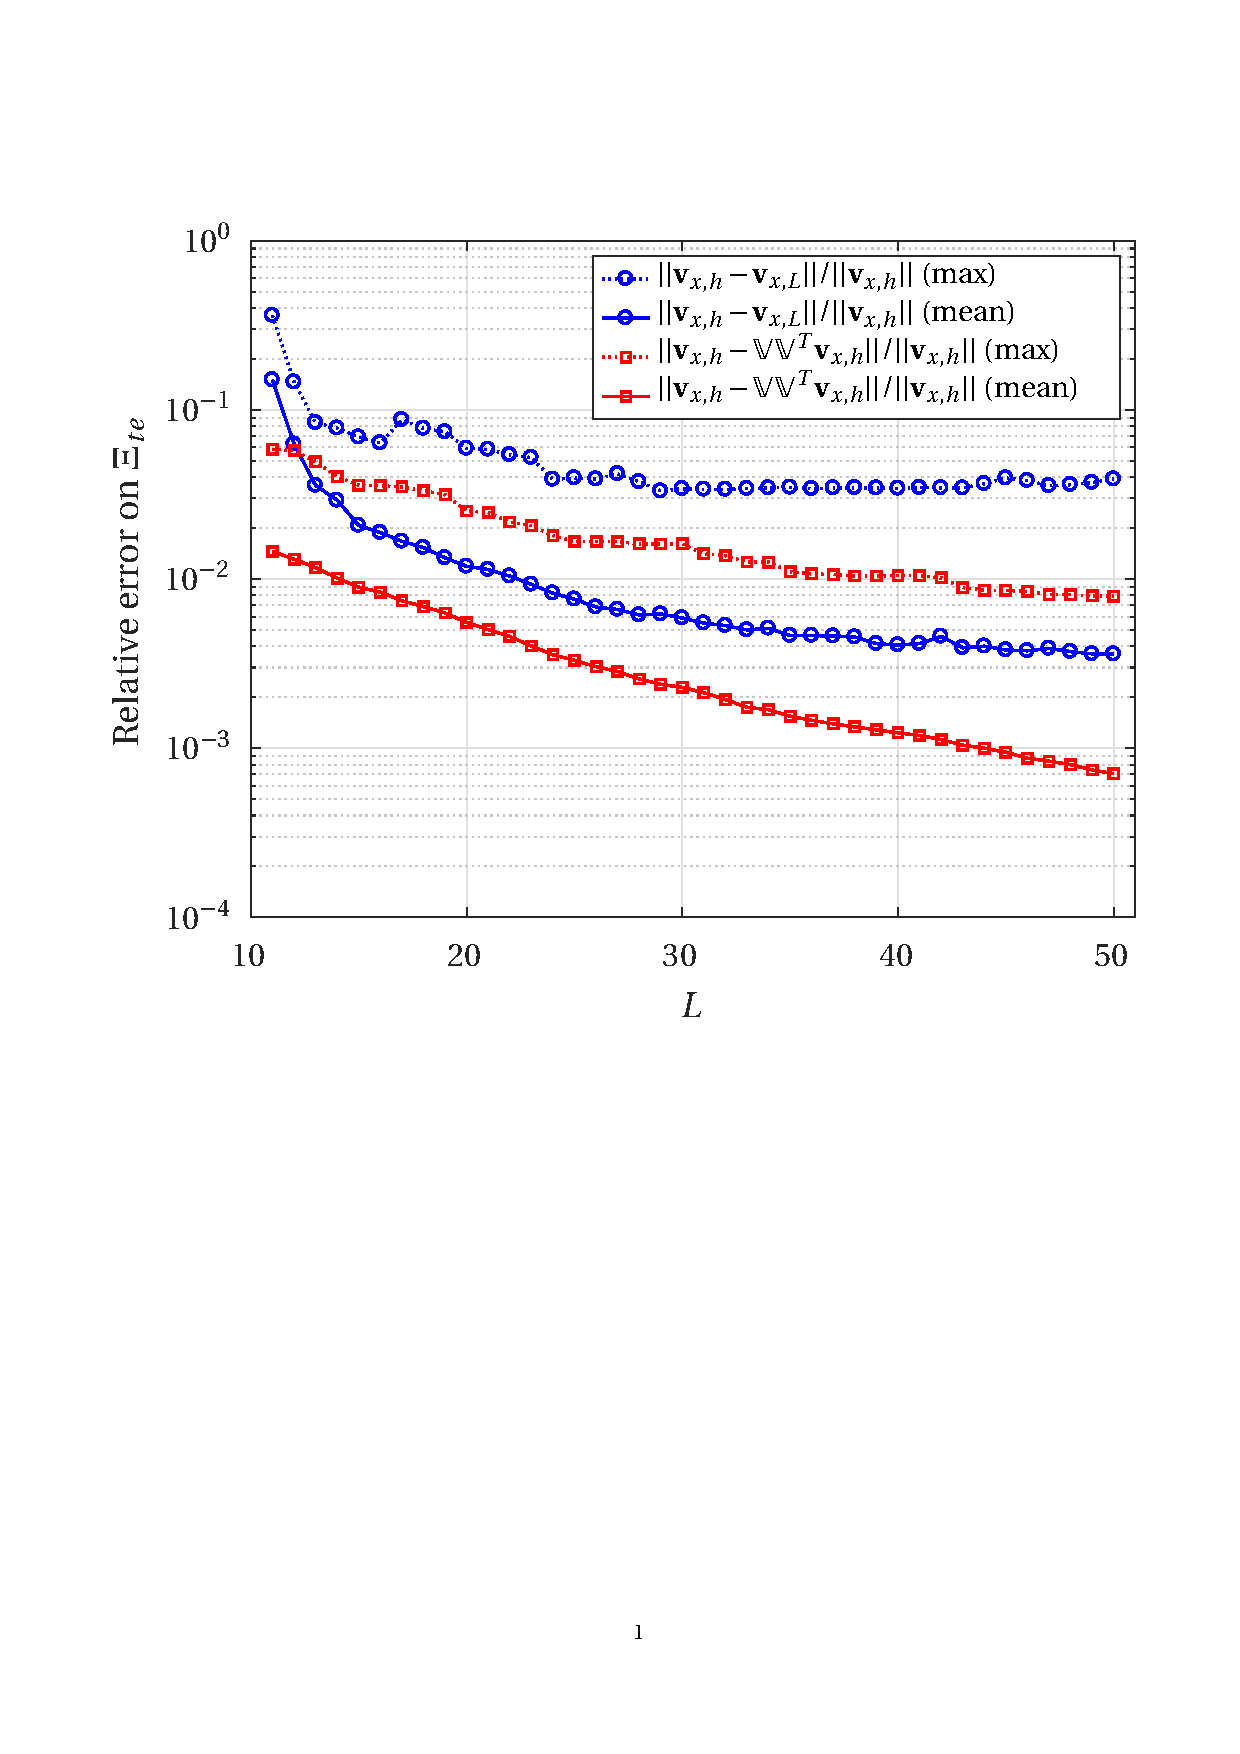
\includegraphics[scale = 0.75, trim = {1.5cm 12cm 1cm 3.5cm}, clip]{dc_200_vx_error_vs_rank}
	\end{figure}
	
	\begin{figure}[H]
		\center
		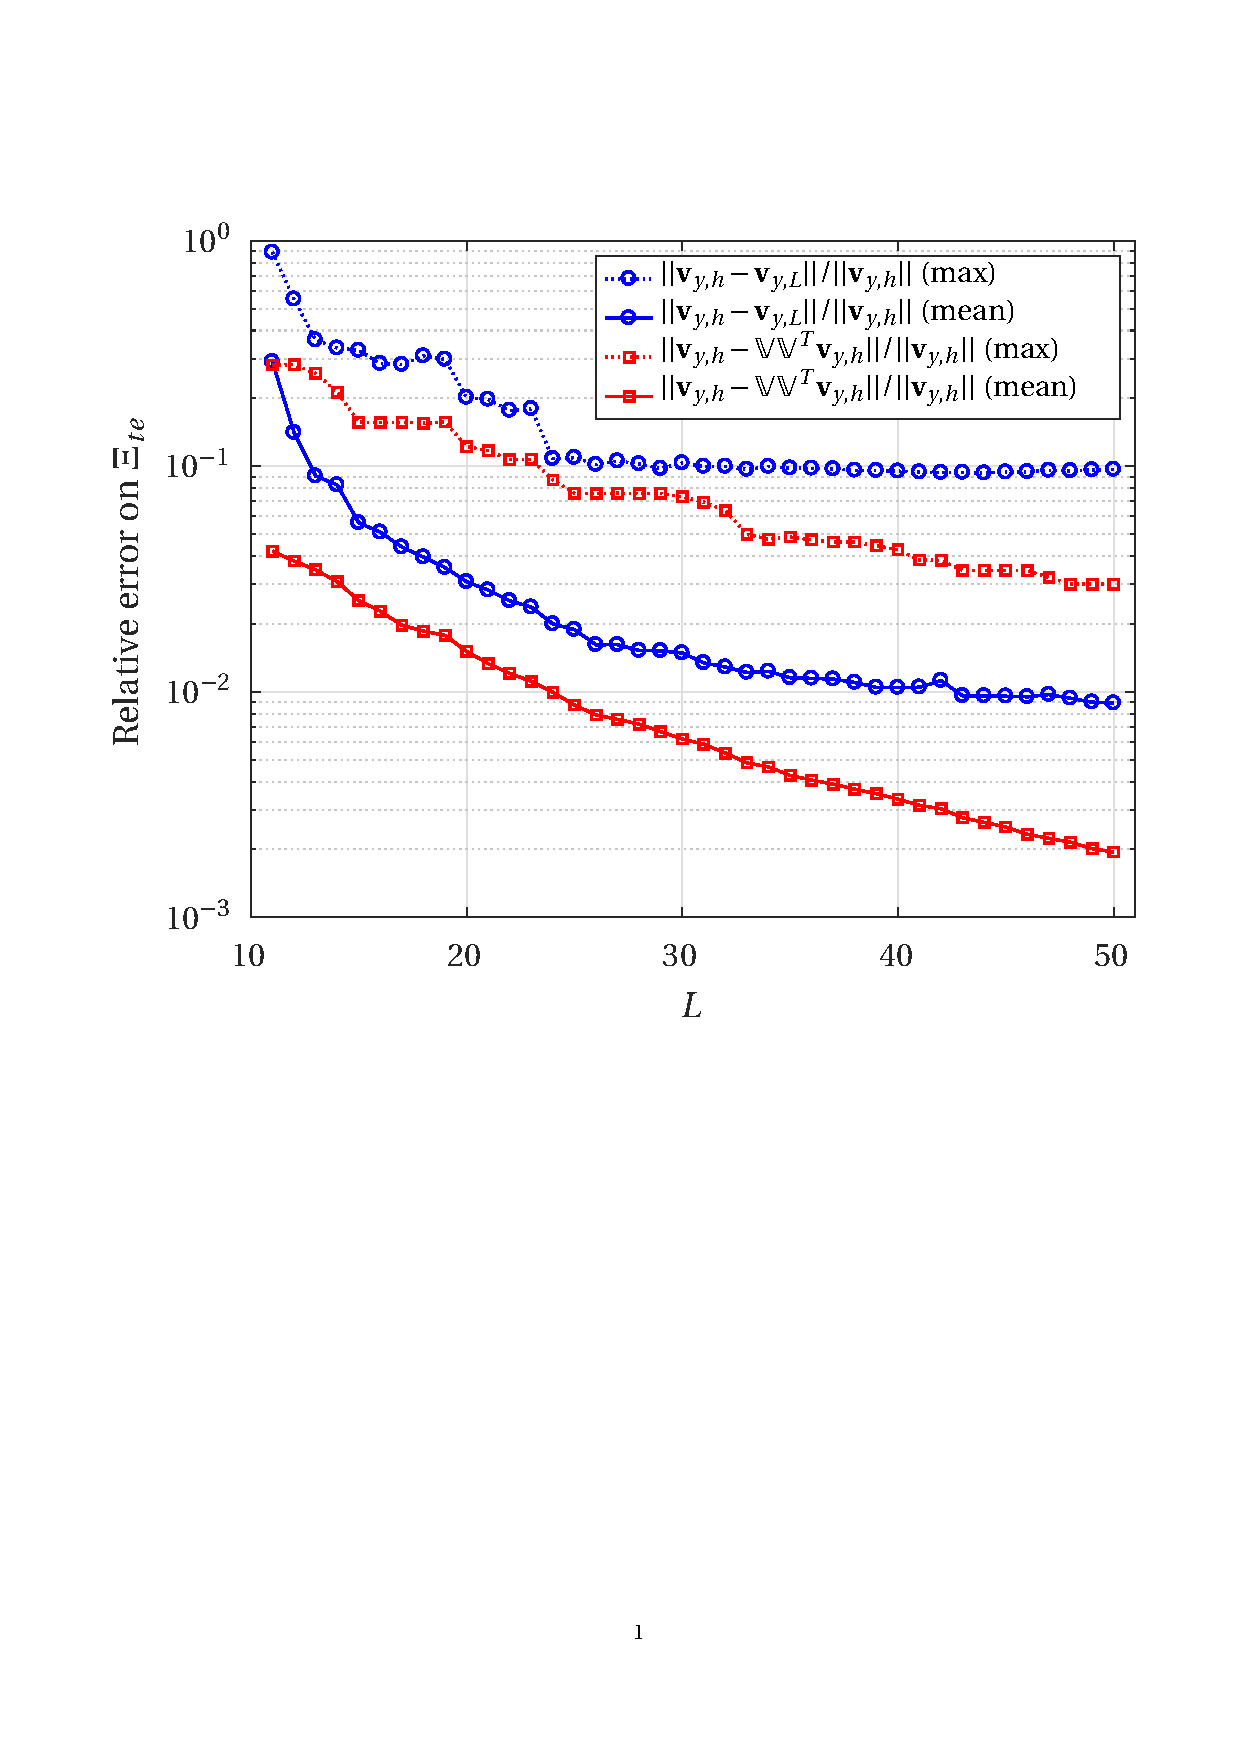
\includegraphics[scale = 0.75, trim = {1.5cm 12cm 1cm 3.5cm}, clip]{dc_200_vy_error_vs_rank}
	\end{figure}
	
	\begin{figure}[H]
		\center
		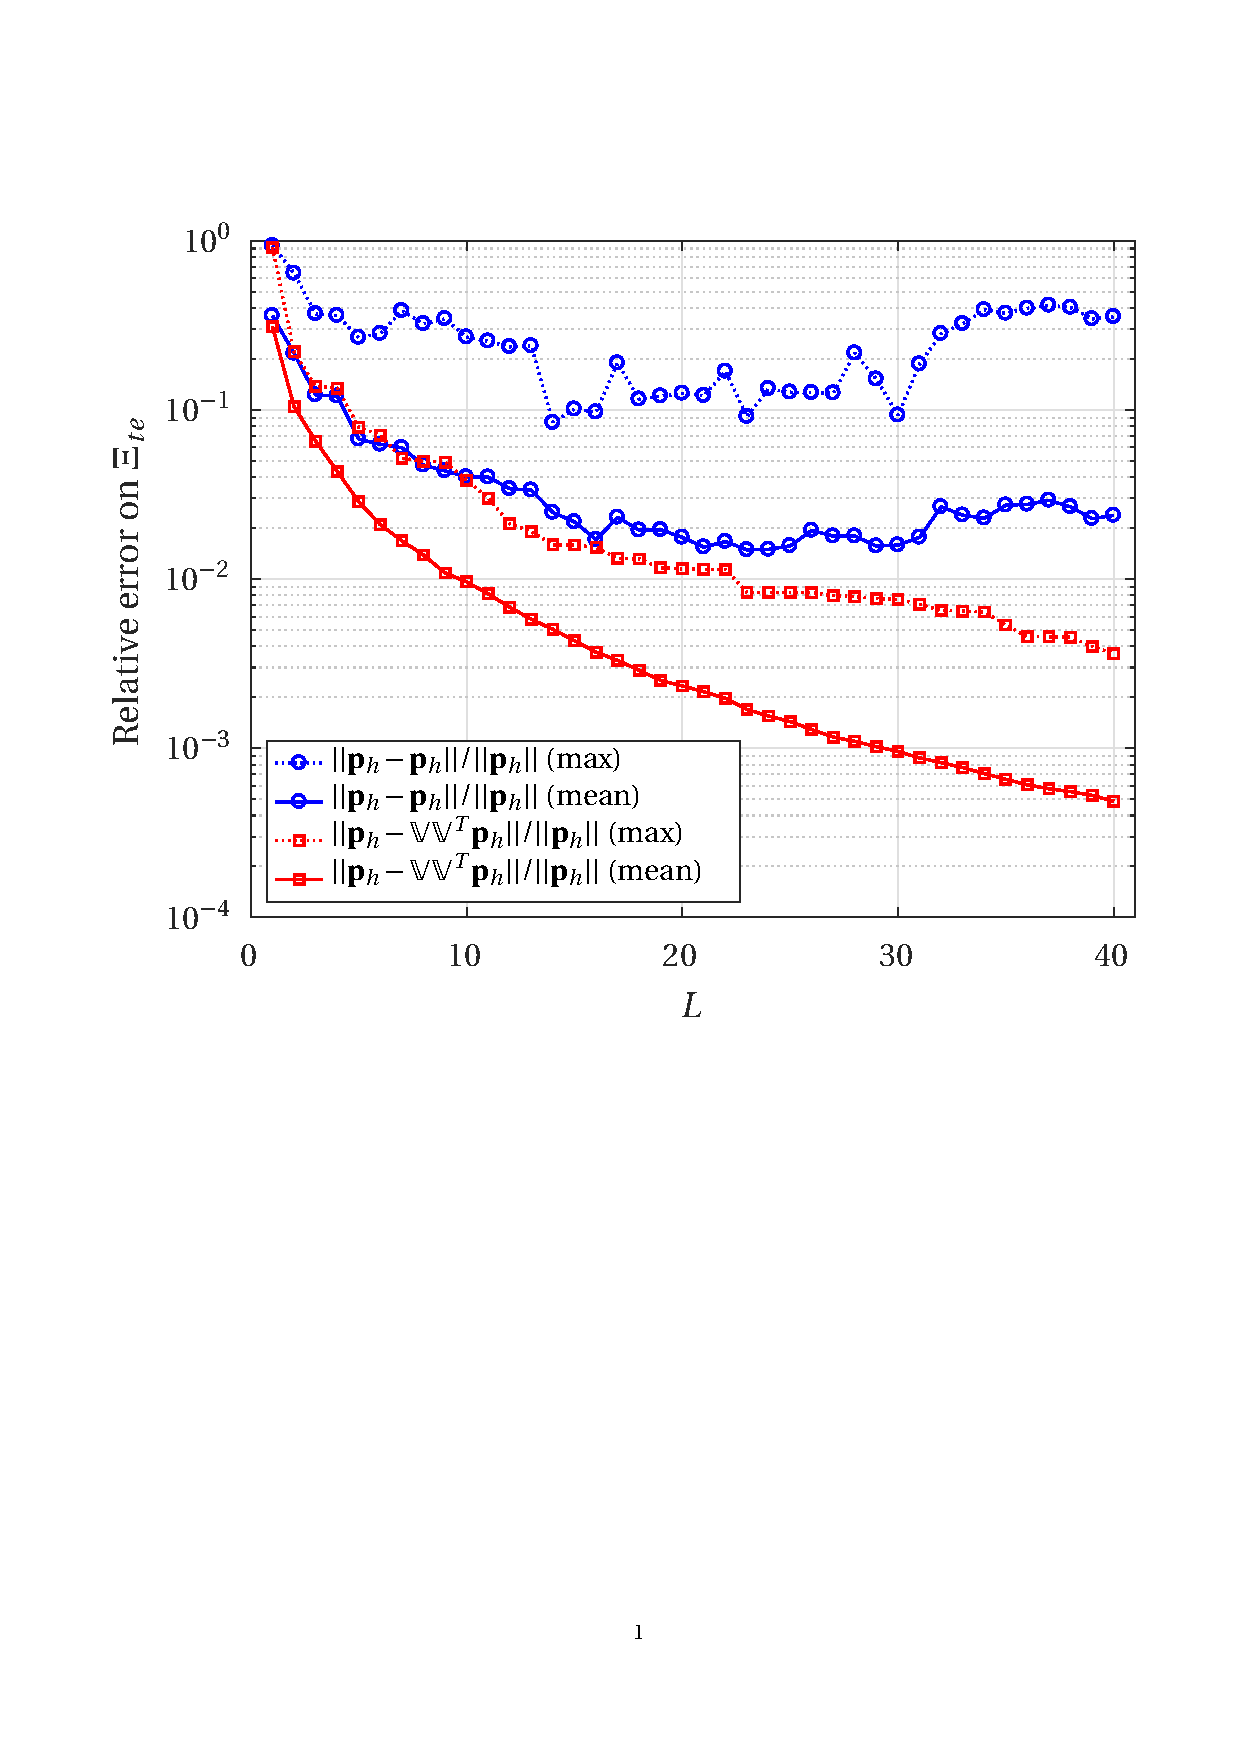
\includegraphics[scale = 0.75, trim = {1.5cm 12cm 1cm 3.5cm}, clip]{dc_200_p_error_vs_rank}
	\end{figure}
	
	\begin{figure}[H]
		\center
		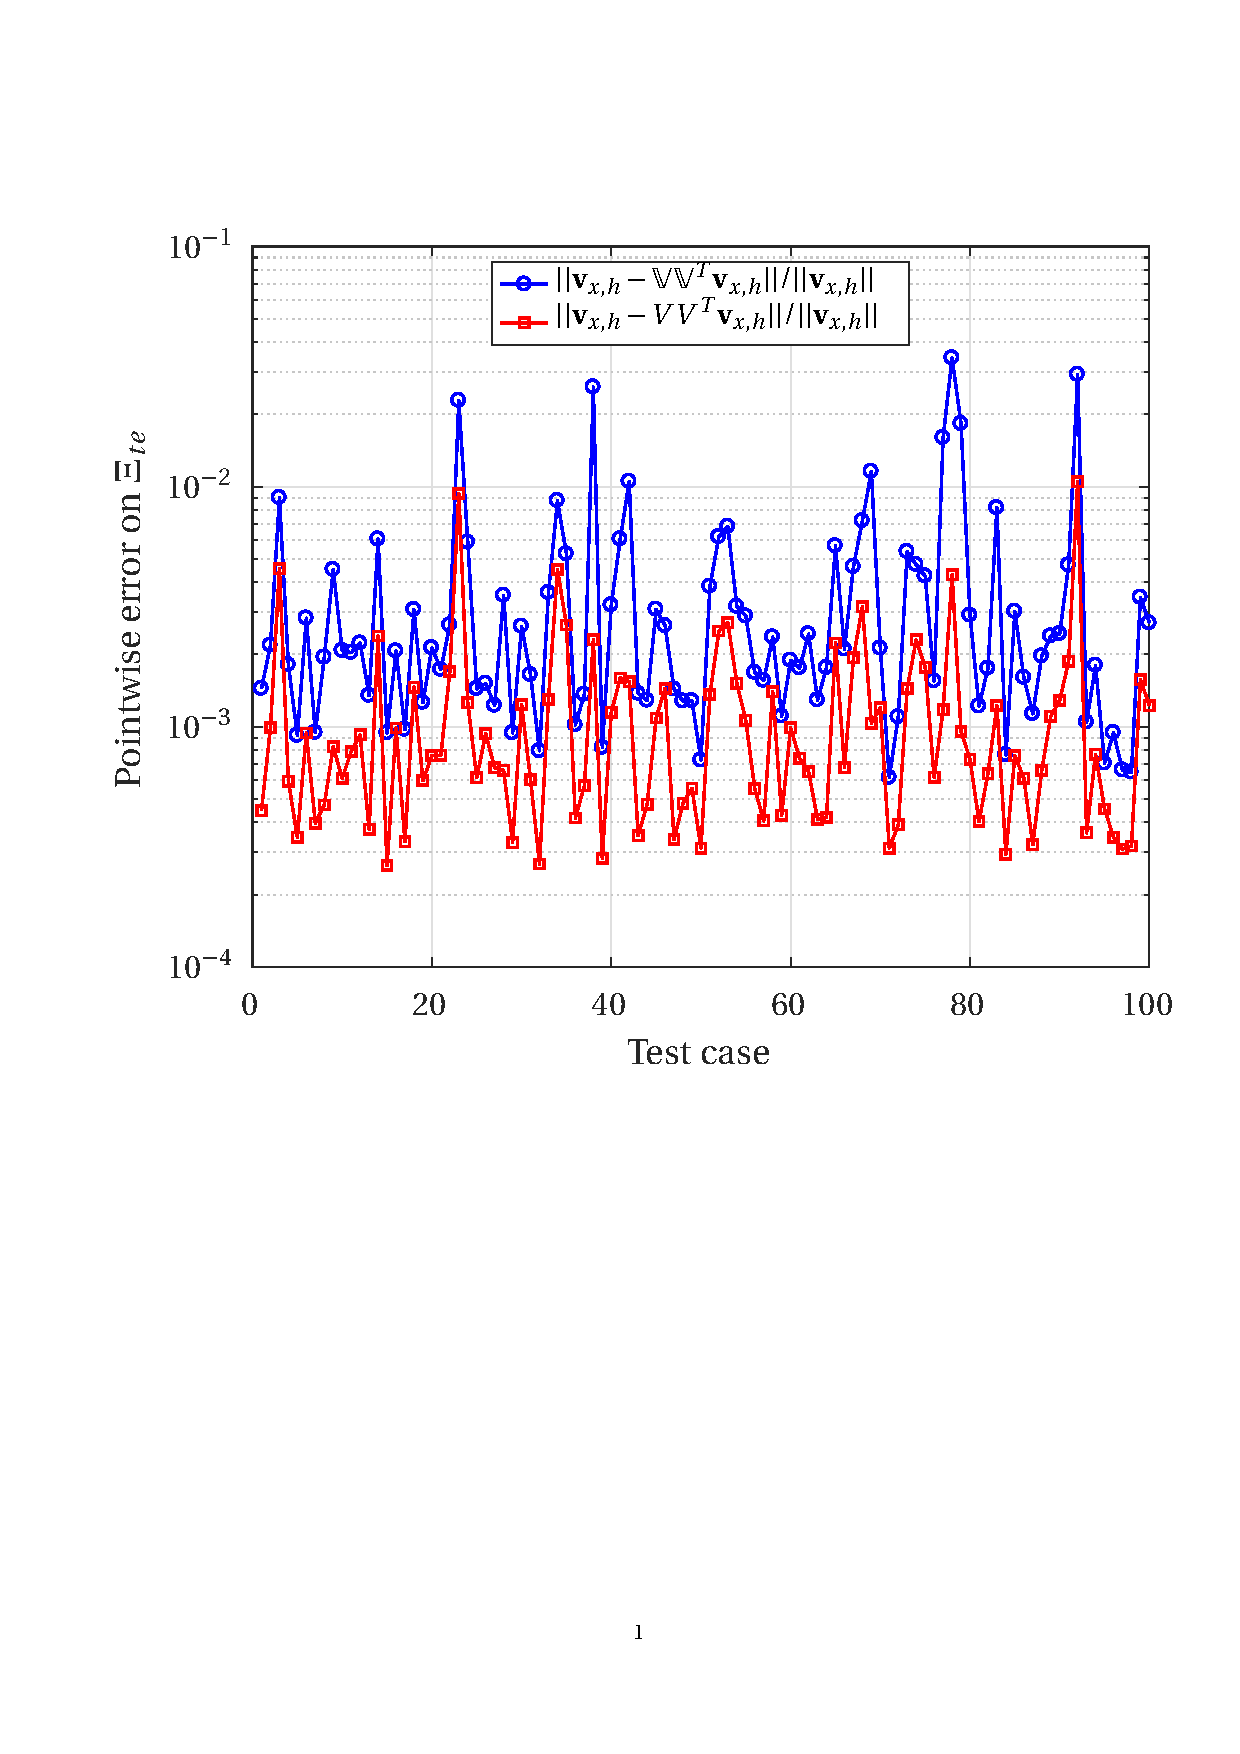
\includegraphics[scale = 0.75, trim = {1.5cm 11cm 1cm 3.5cm}, clip]{dc_200_vx_pointwise_error}
	\end{figure}
	
	\begin{figure}[H]
		\center
		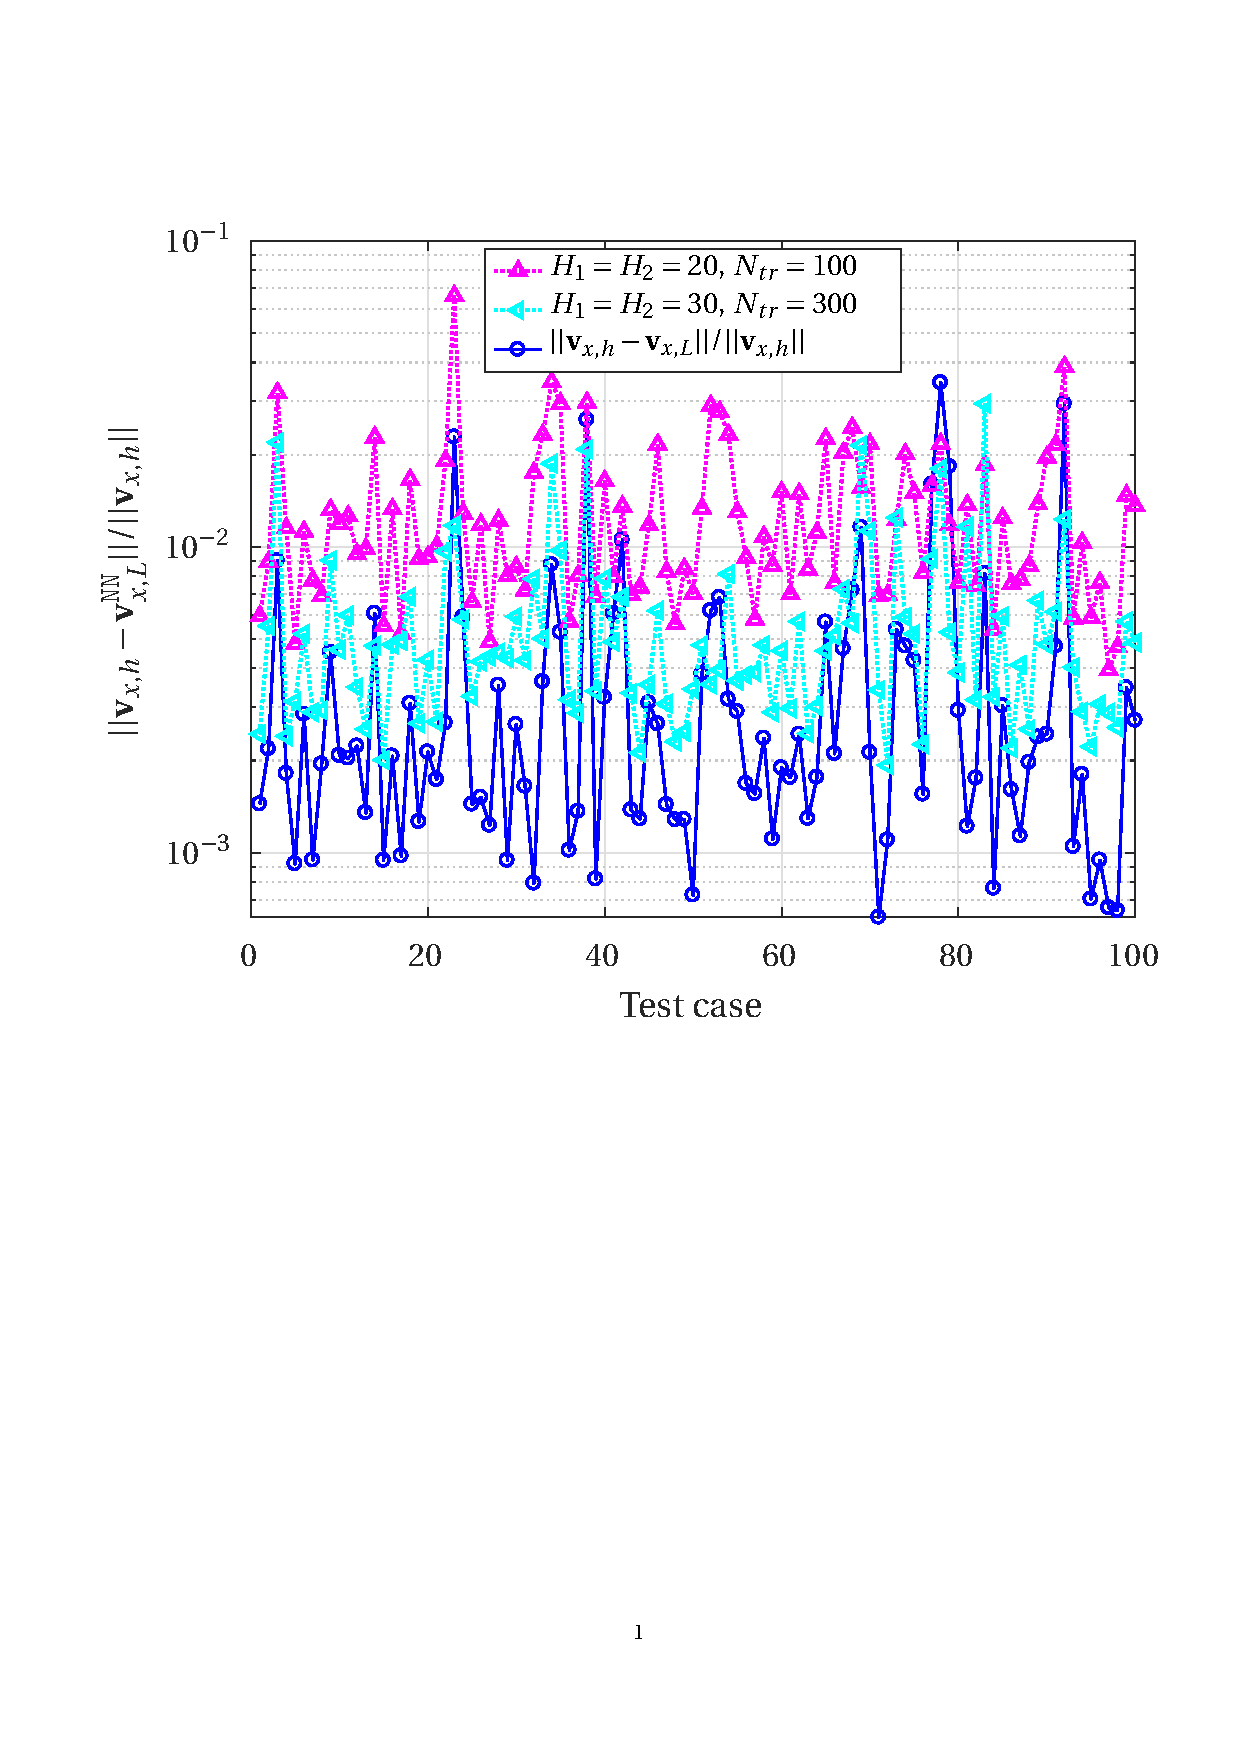
\includegraphics[scale = 0.75, trim = {1.5cm 12cm 1cm 3.5cm}, clip]{dc_200_vx_pointwise_error_nn}
	\end{figure}
	
	\begin{figure}[H]
		\center
		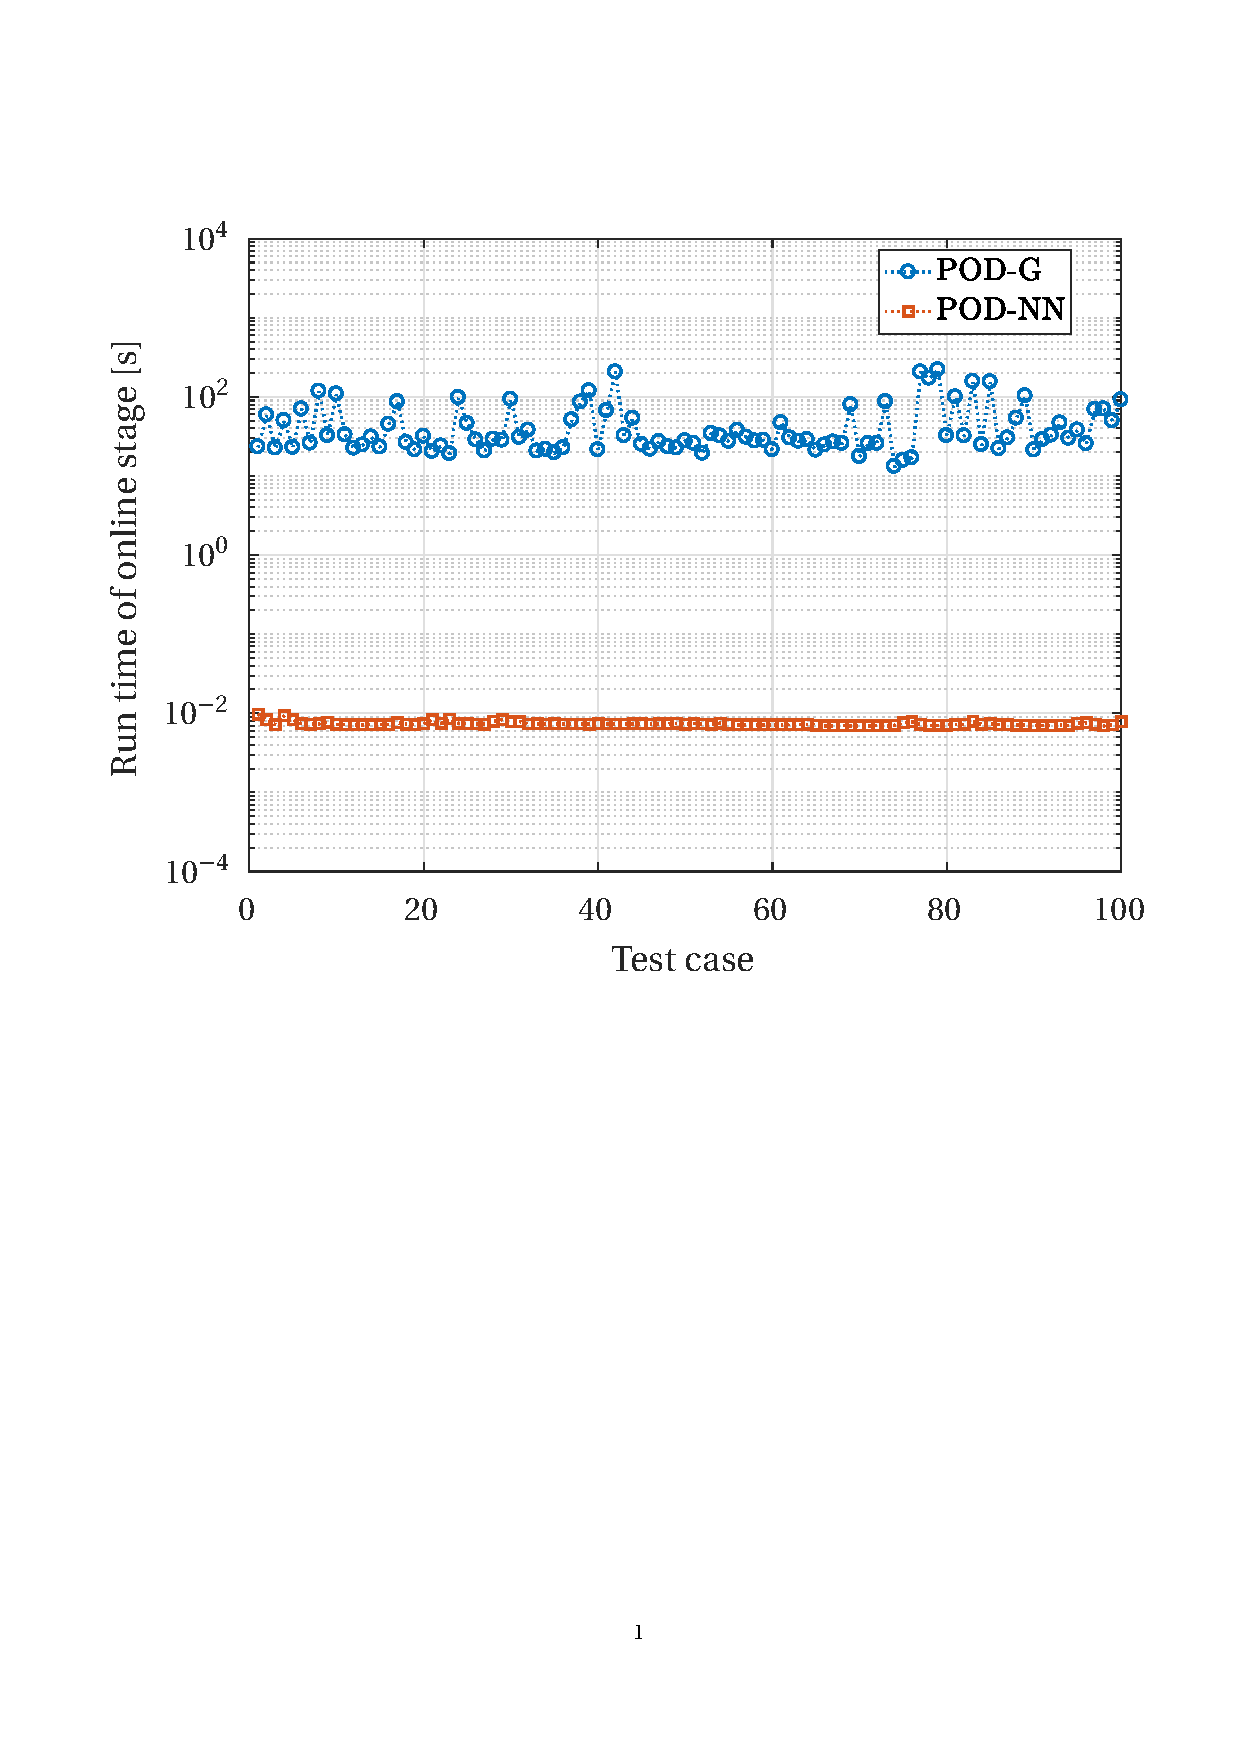
\includegraphics[scale = 0.75, trim = {1.5cm 12cm 1cm 3.5cm}, clip]{dc_200_time}
	\end{figure}
	
	\begin{figure}[H]
		\center
		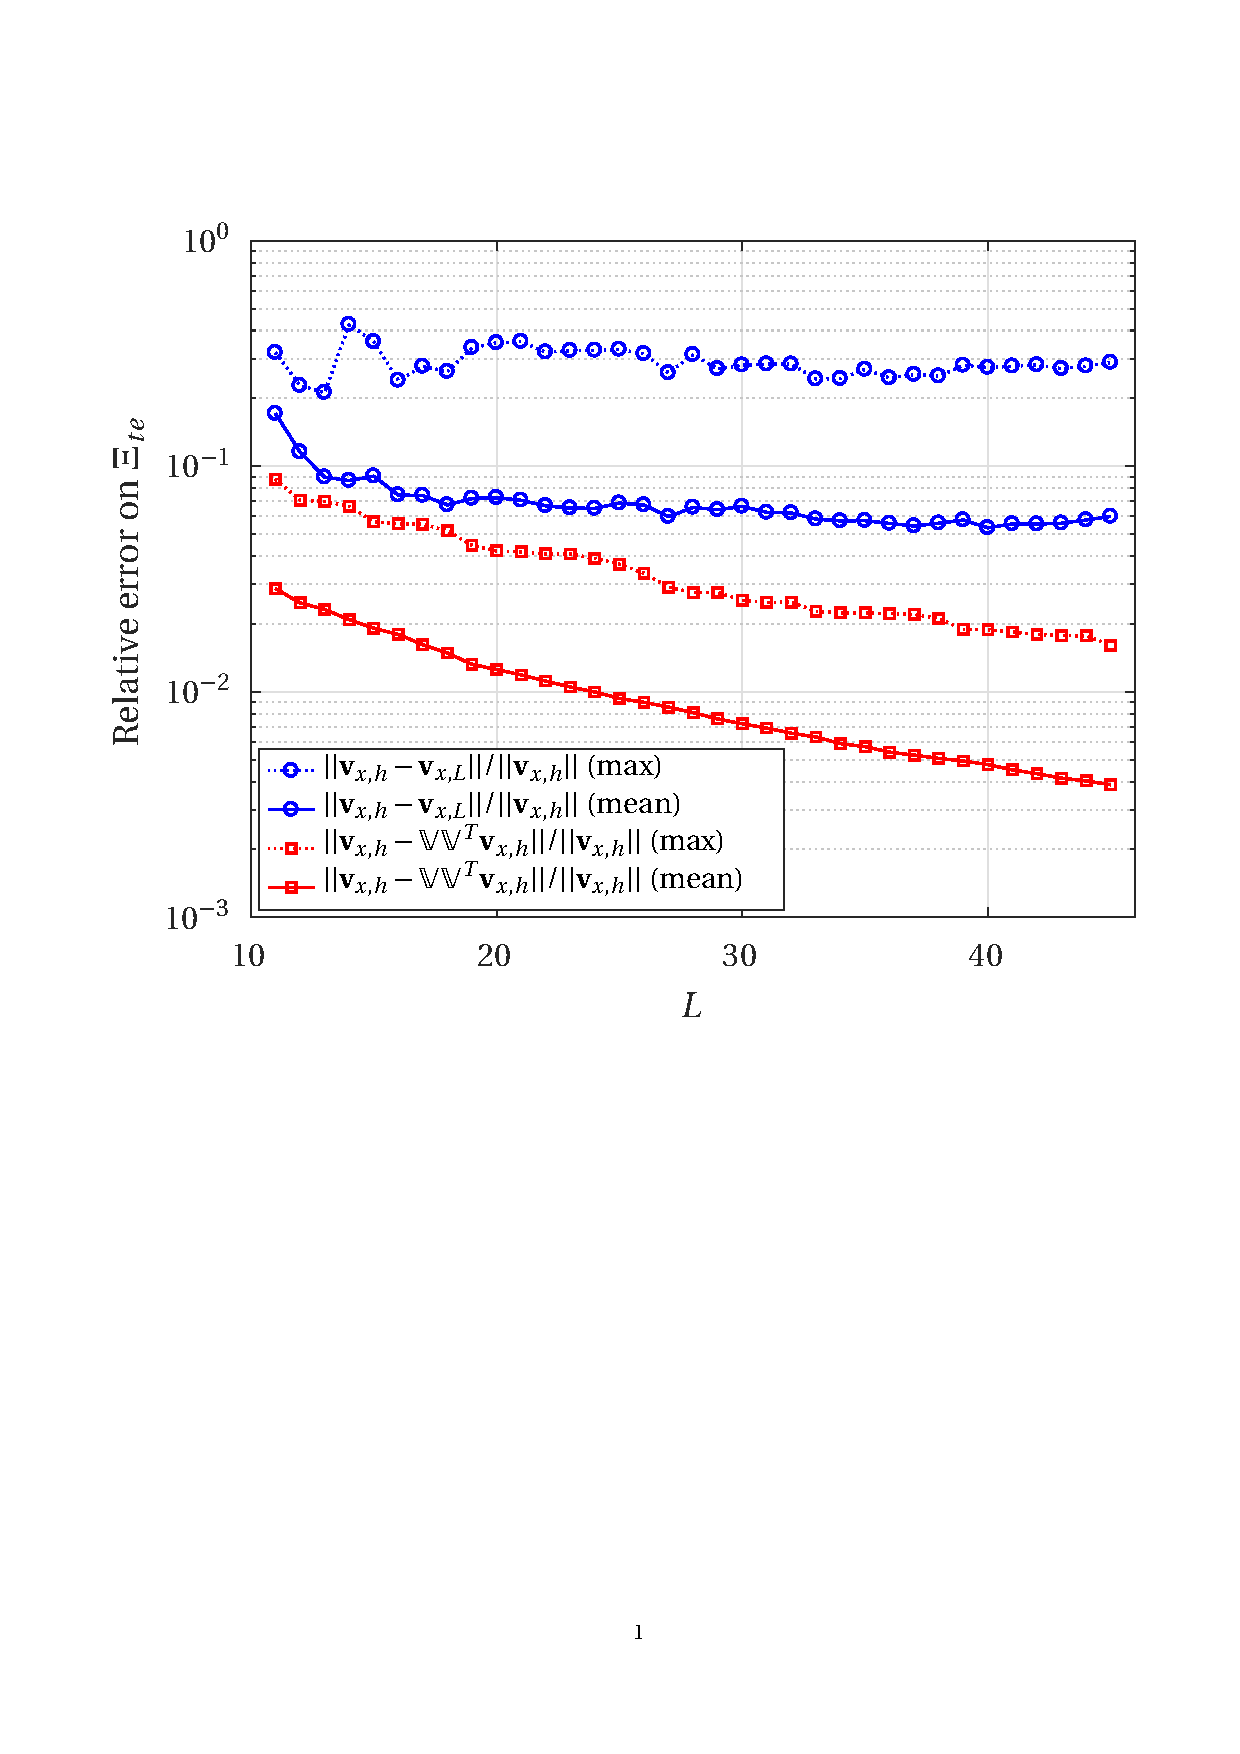
\includegraphics[scale = 0.75, trim = {1.5cm 12cm 1cm 3.5cm}, clip]{dc_400_vx_error_vs_rank}
	\end{figure}
	
	\begin{figure}[H]
		\center
		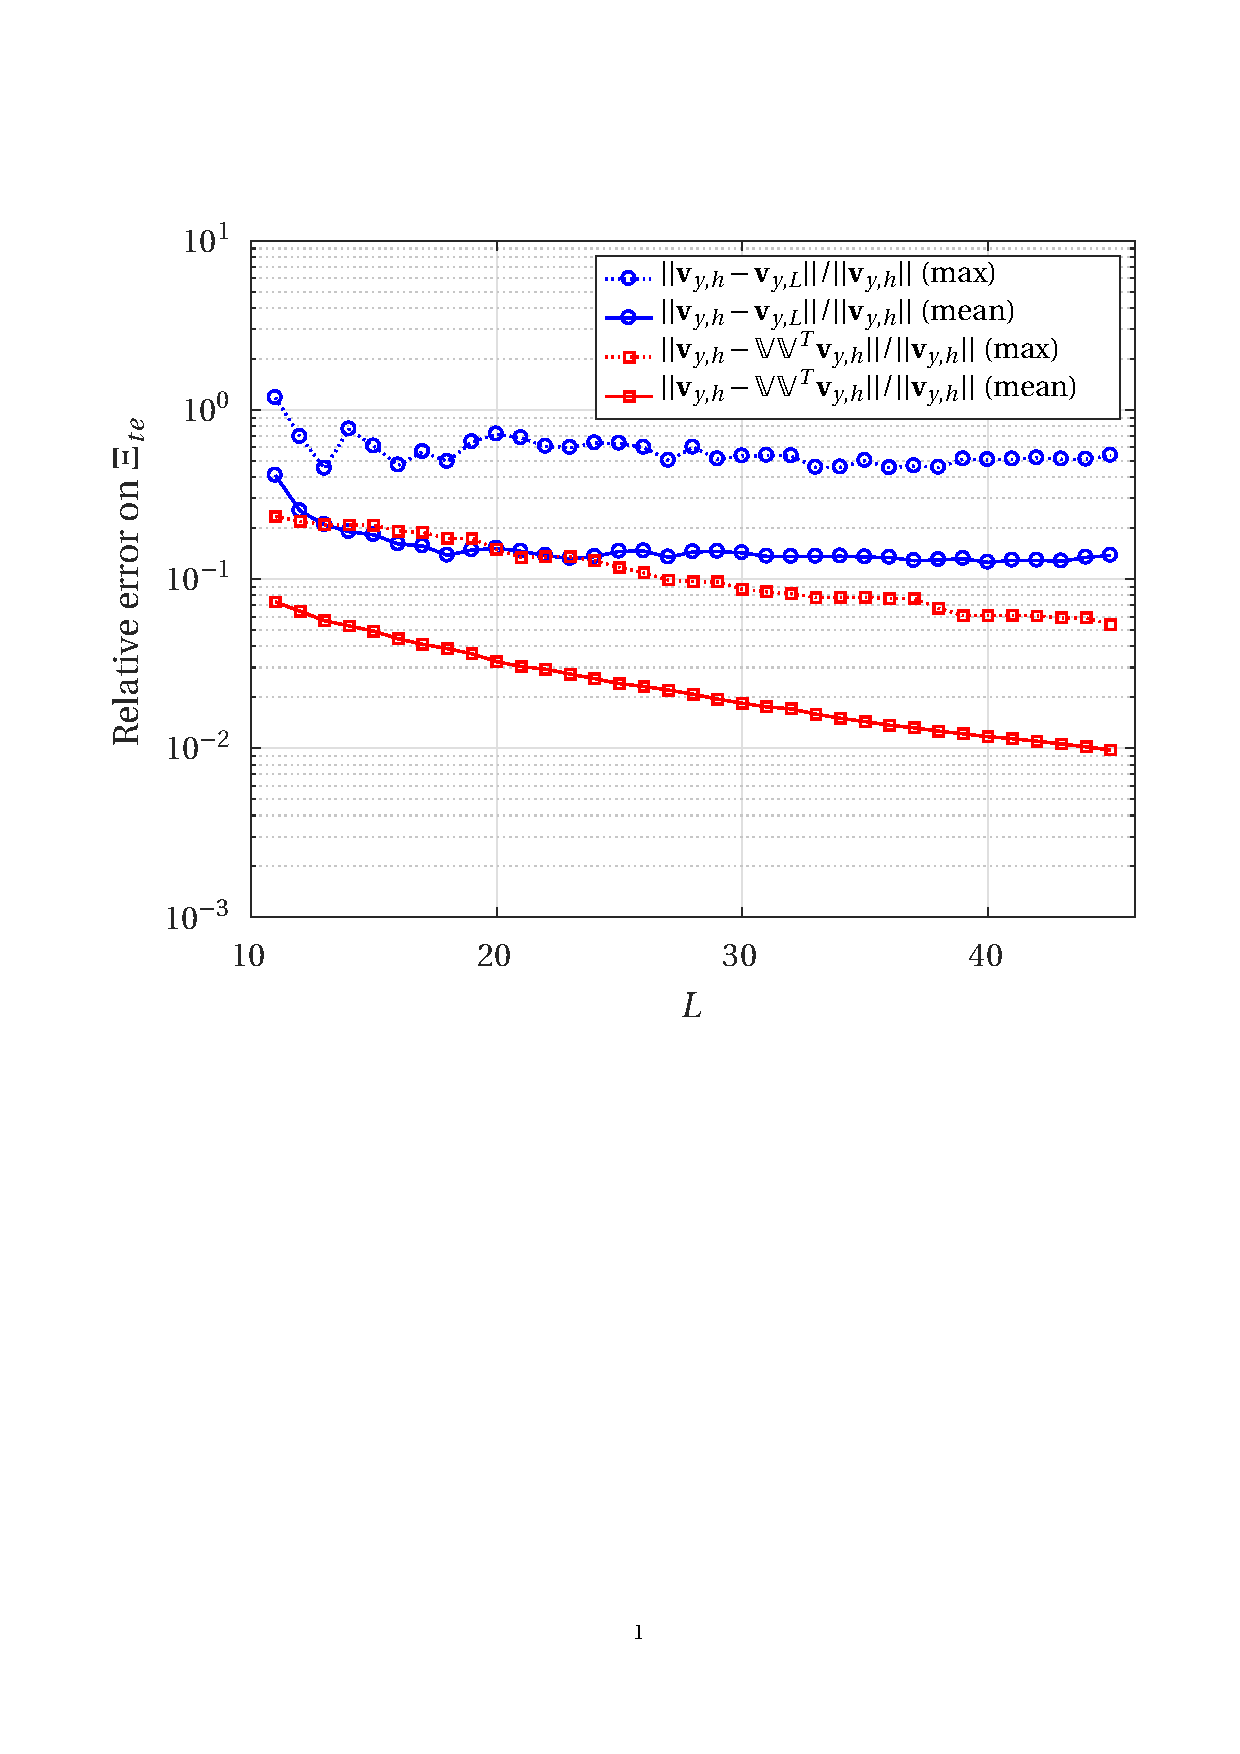
\includegraphics[scale = 0.75, trim = {1.5cm 12cm 1cm 3.5cm}, clip]{dc_400_vy_error_vs_rank}
	\end{figure}
	
	\begin{figure}[H]
		\center
		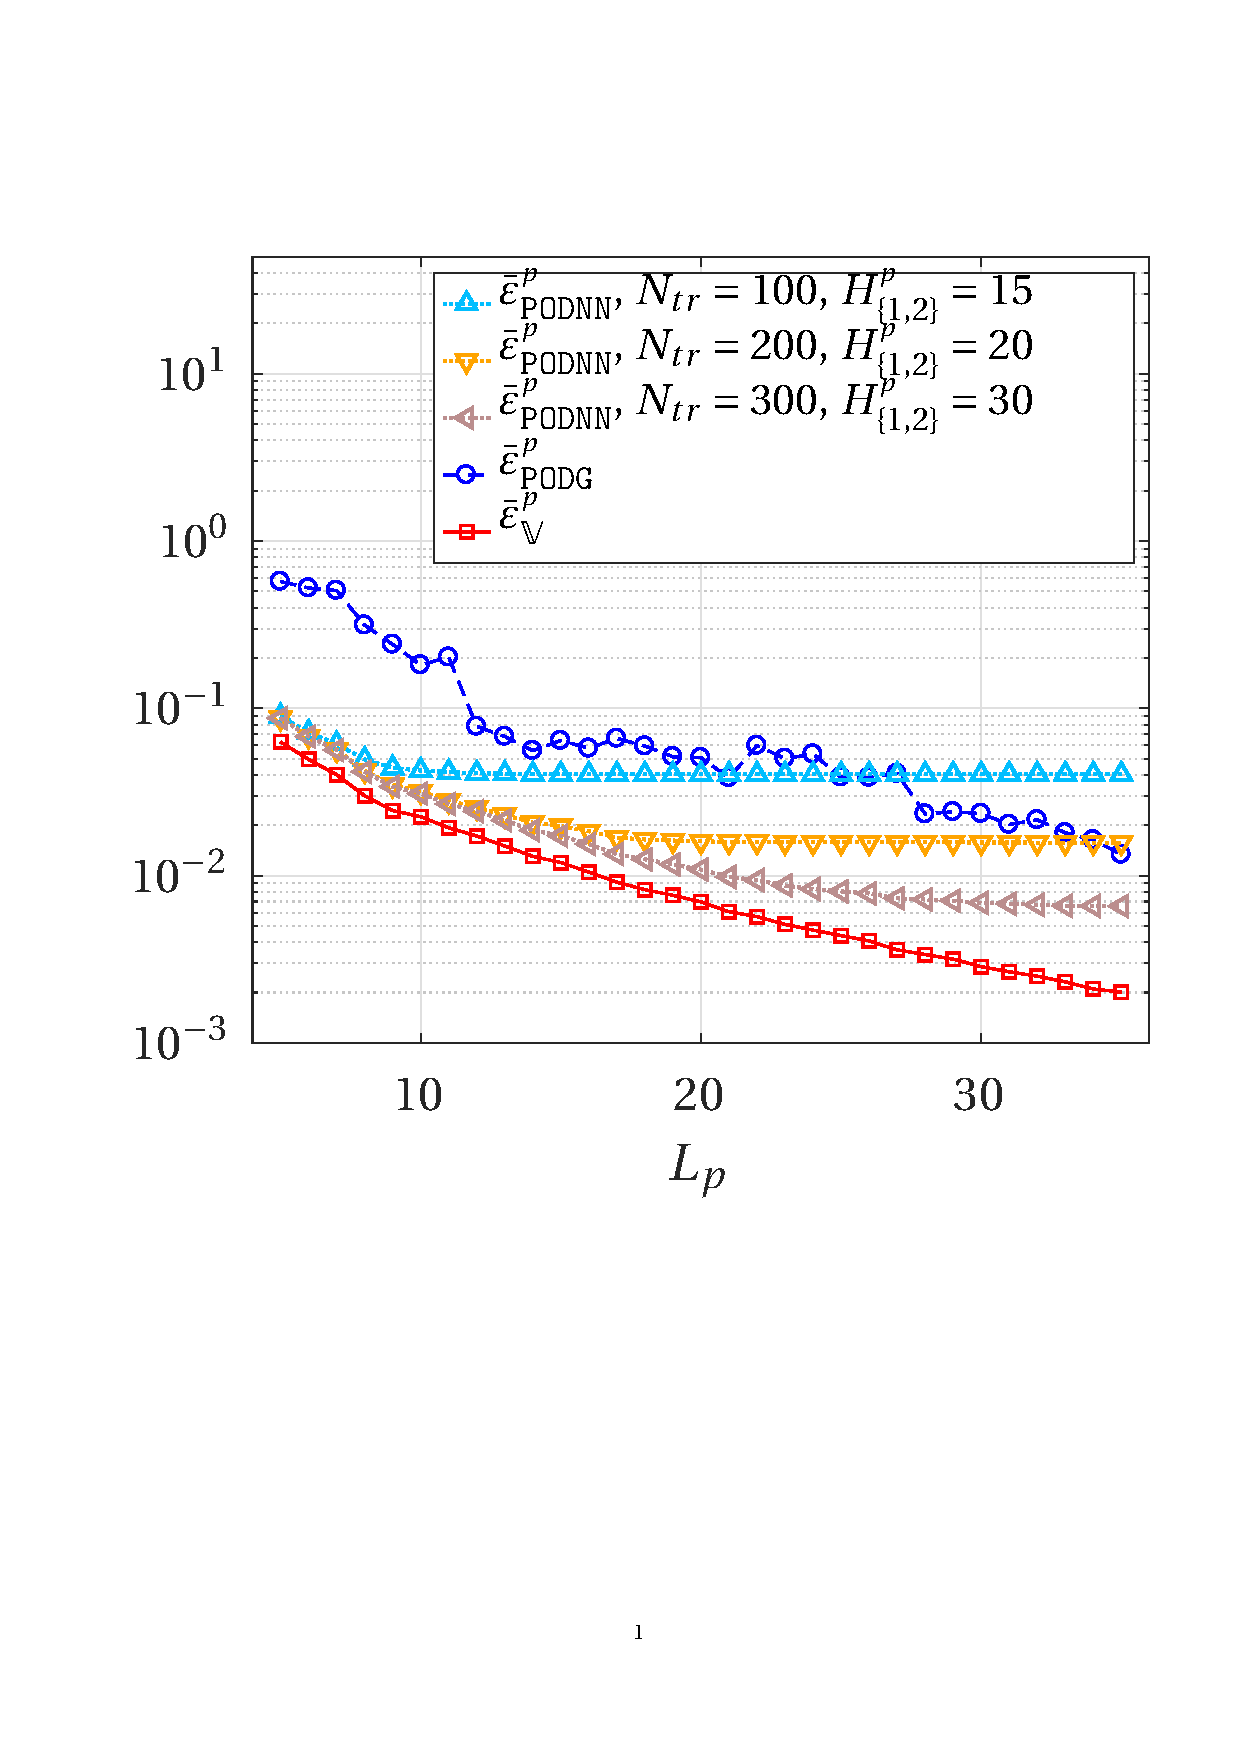
\includegraphics[scale = 0.75, trim = {1.5cm 11cm 1cm 3.5cm}, clip]{dc_400_p_error_vs_rank}
	\end{figure}
	
	\begin{figure}[H]
		\center
		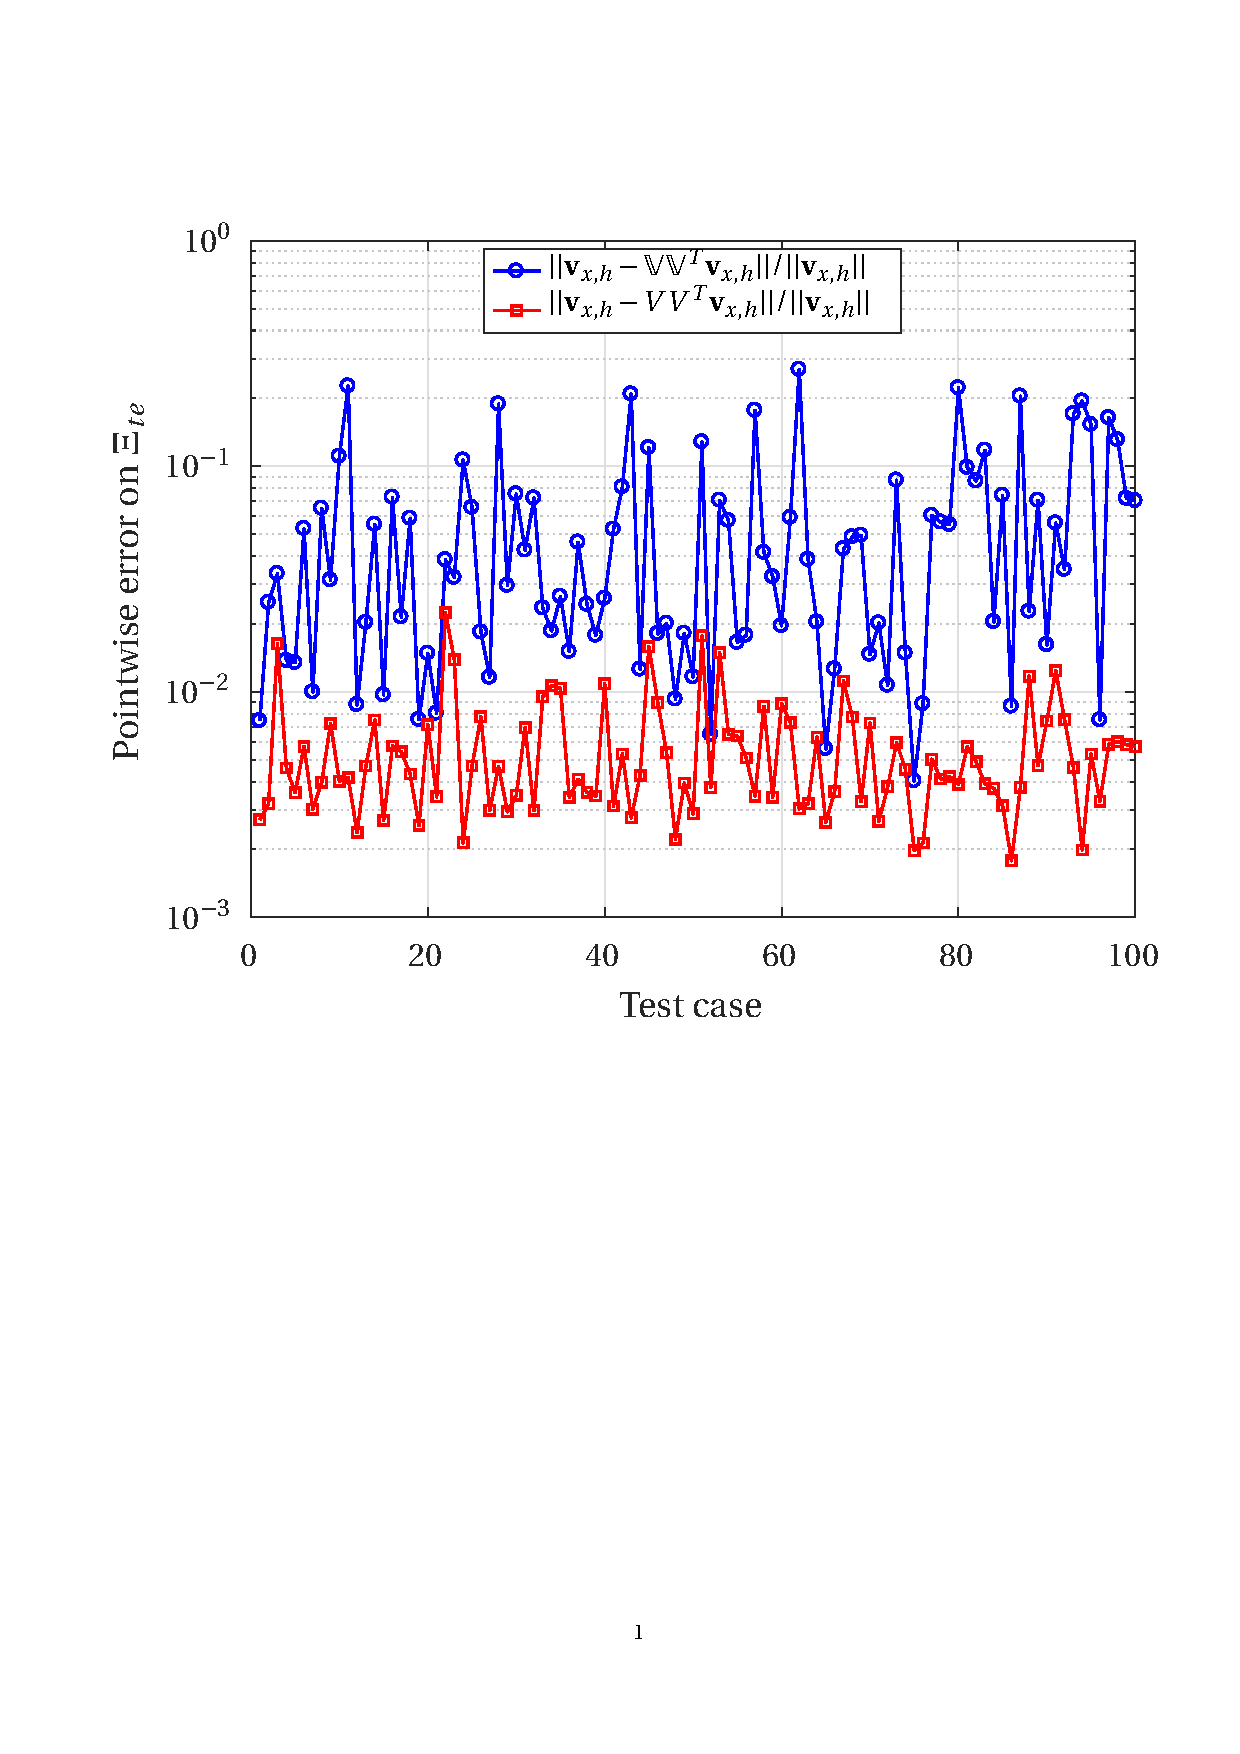
\includegraphics[scale = 0.75, trim = {1.5cm 11cm 1cm 3.5cm}, clip]{dc_400_vx_pointwise_error}
	\end{figure}
	
	\begin{figure}[H]
		\center
		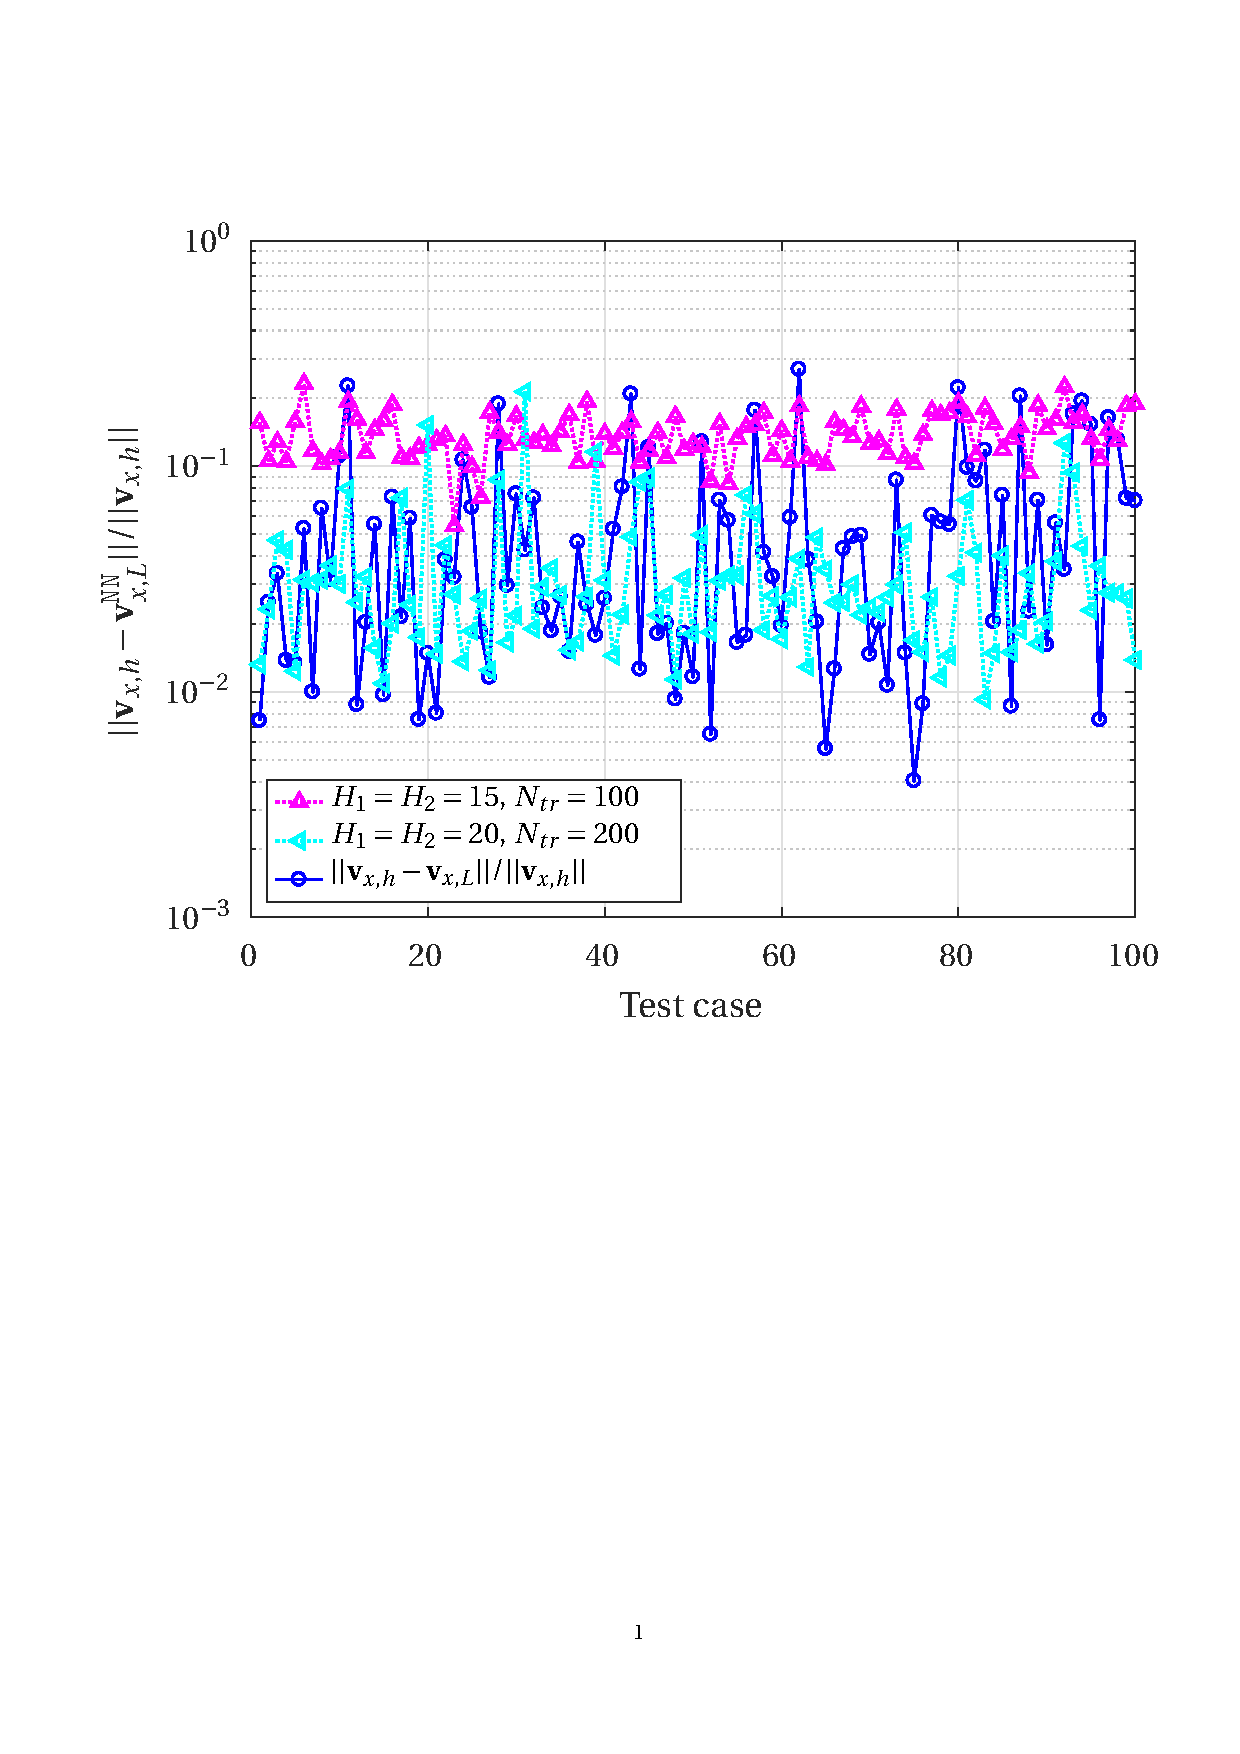
\includegraphics[scale = 0.75, trim = {1.5cm 12cm 1cm 3.5cm}, clip]{dc_400_vx_pointwise_error_nn}
	\end{figure}
	
	\begin{figure}[H]
		\center
		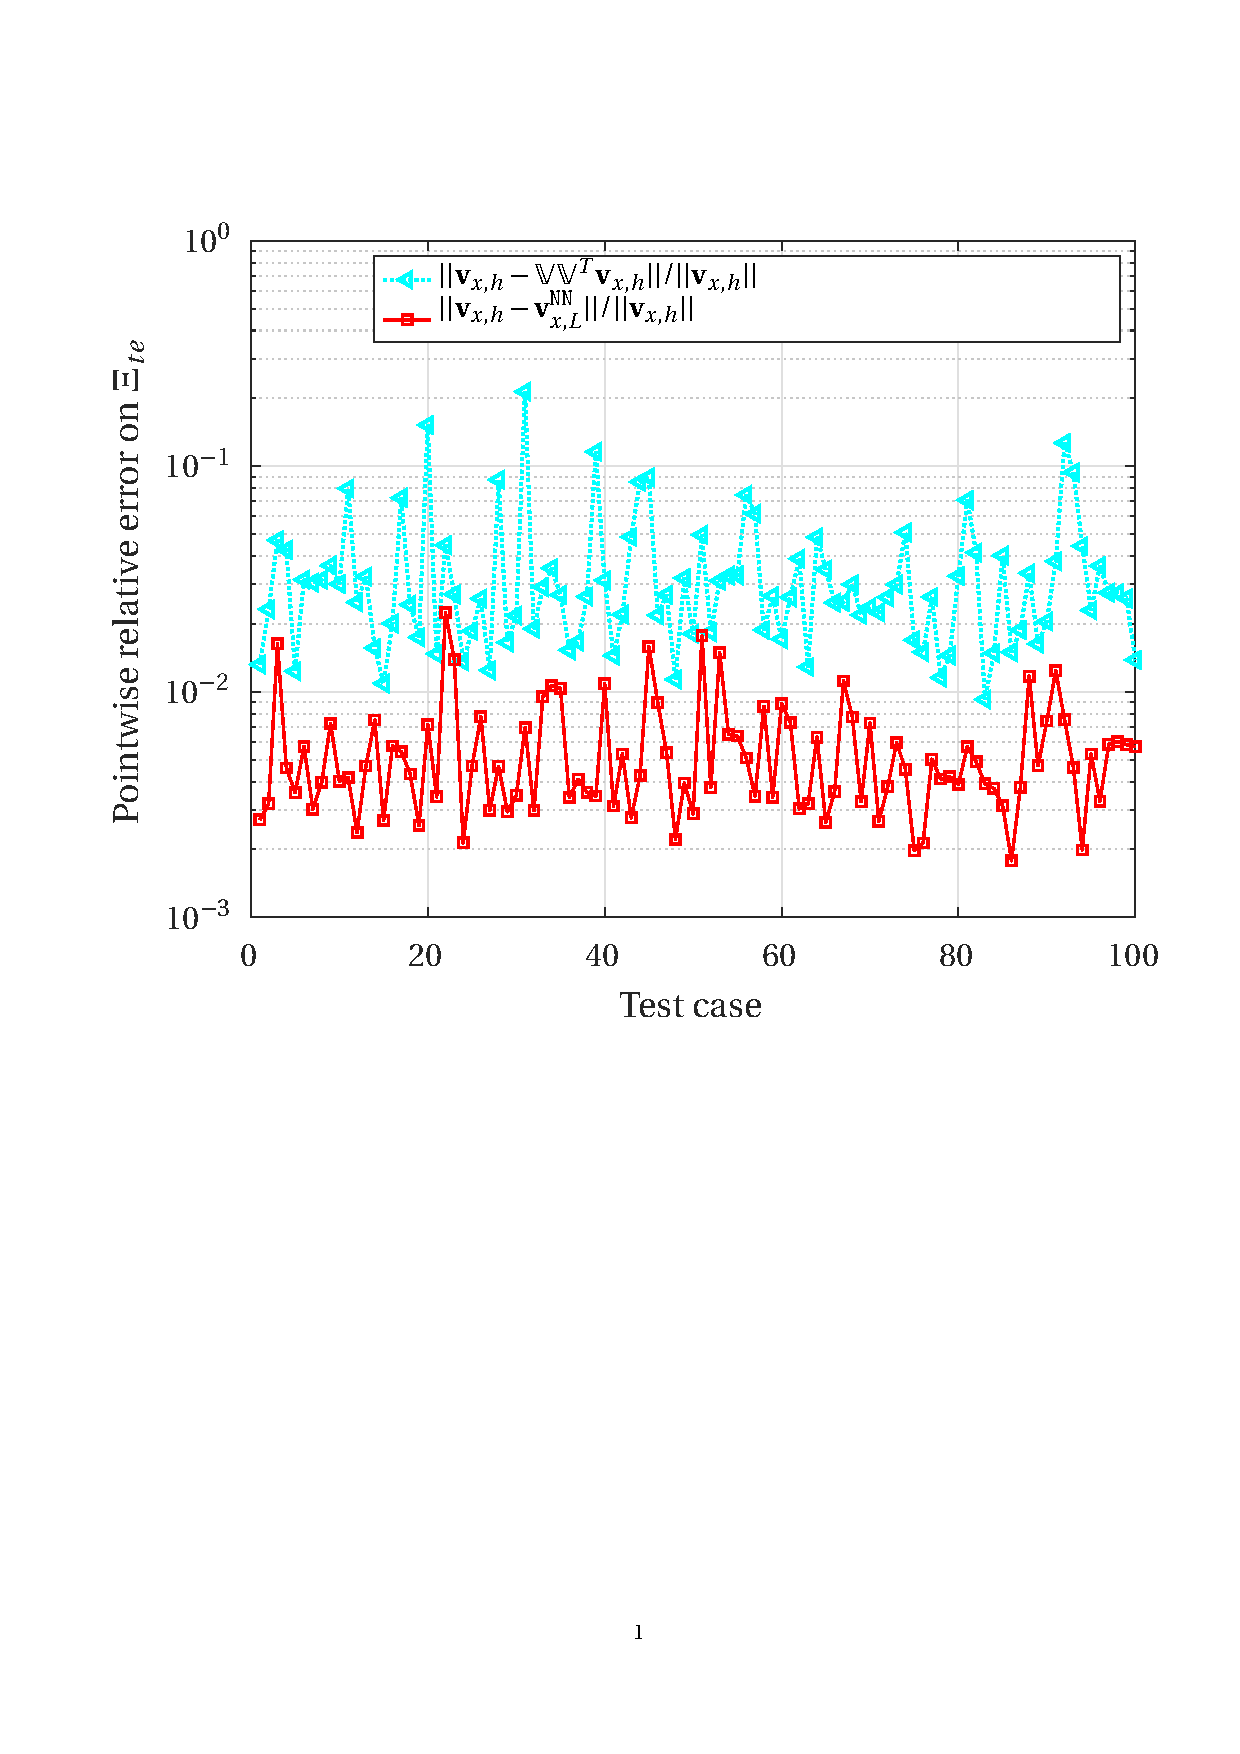
\includegraphics[scale = 0.75, trim = {1.5cm 12cm 1cm 3.5cm}, clip]{dc_400_vx_pointwise_error_nn_bis}
	\end{figure}
	
	\begin{figure}[H]
		\center
		\subfloat[Truth]{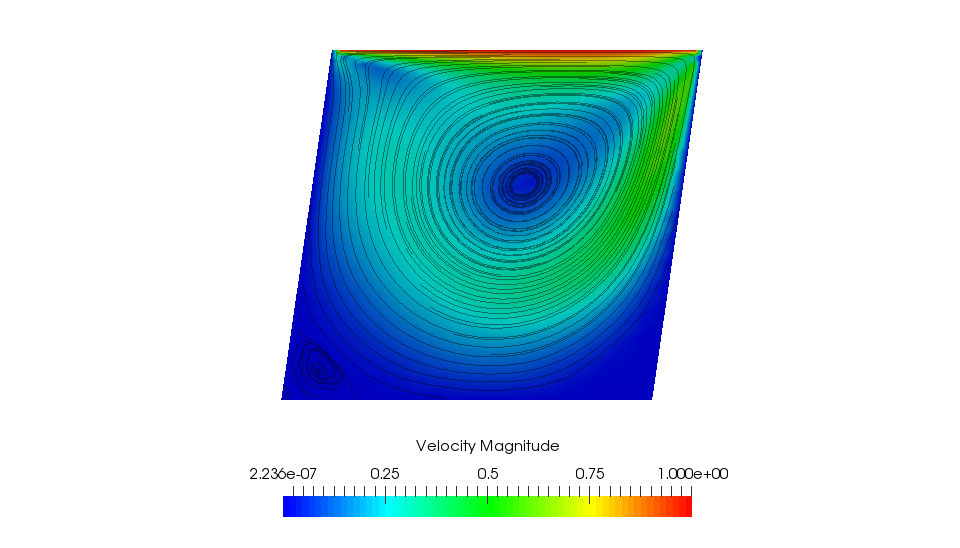
\includegraphics[scale = 0.4, trim = {7.5cm 0 7.5cm 0}, clip]{dc_400_test1_full}}
		\subfloat[Projection]{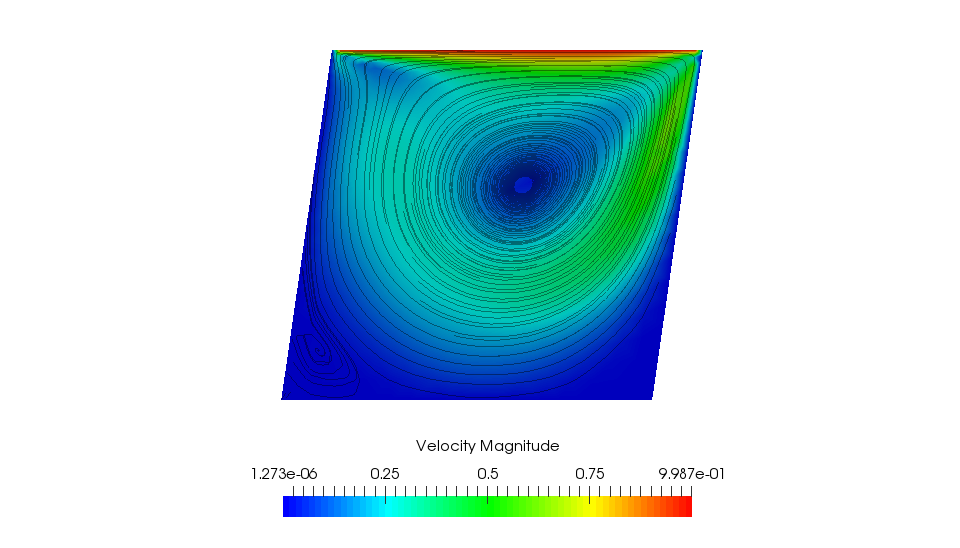
\includegraphics[scale = 0.4, trim = {7.5cm 0 7.5cm 0}, clip]{dc_400_test1_proj}} \\
		\subfloat[POD-G]{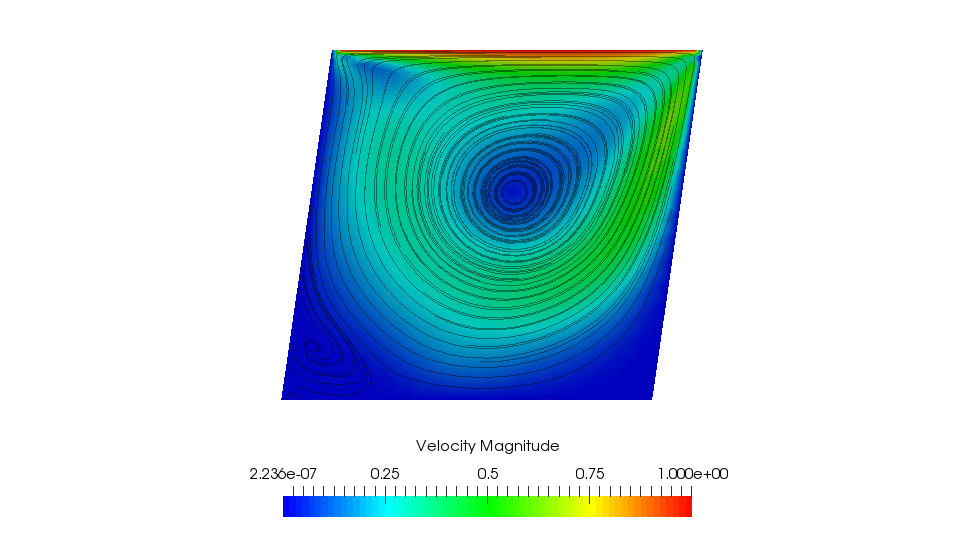
\includegraphics[scale = 0.4, trim = {7.5cm 0 7.5cm 0}, clip]{dc_400_test1_podg}}
		\subfloat[POD-N]{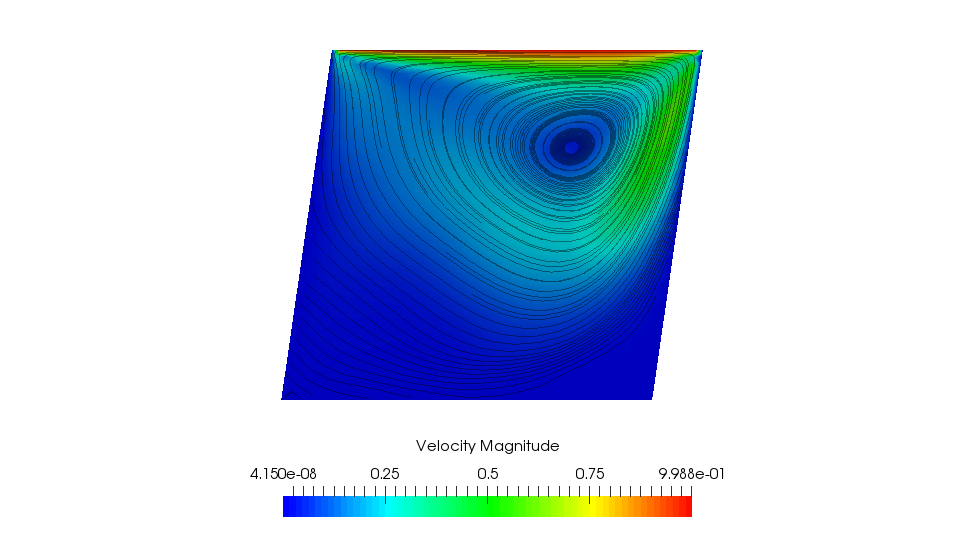
\includegraphics[scale = 0.4, trim = {7.5cm 0 7.5cm 0}, clip]{dc_400_test1_podnn}}
	\end{figure}
	
	\begin{figure}[H]
		\center
		\subfloat[Truth]{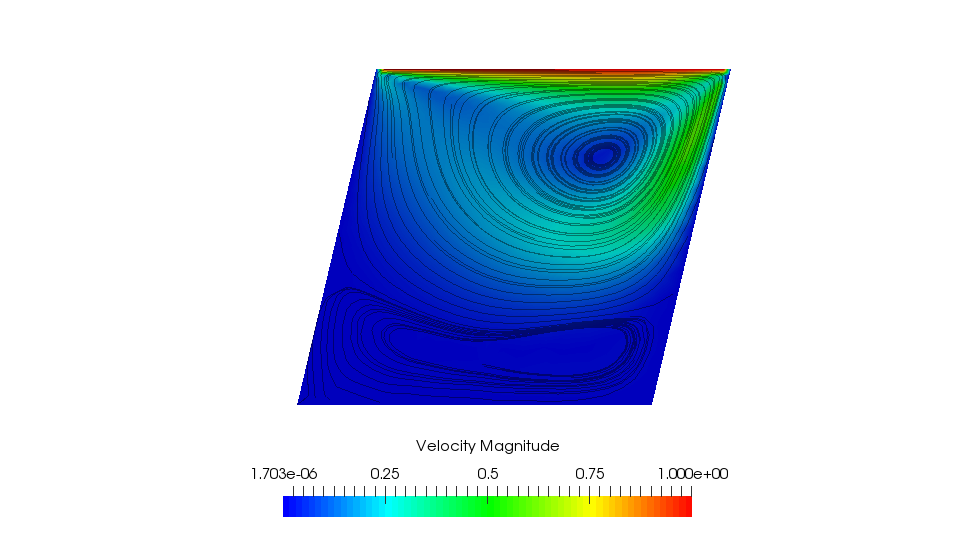
\includegraphics[scale = 0.4, trim = {7.5cm 0 7.5cm 0}, clip]{dc_400_test2_full}}
		\subfloat[Projection]{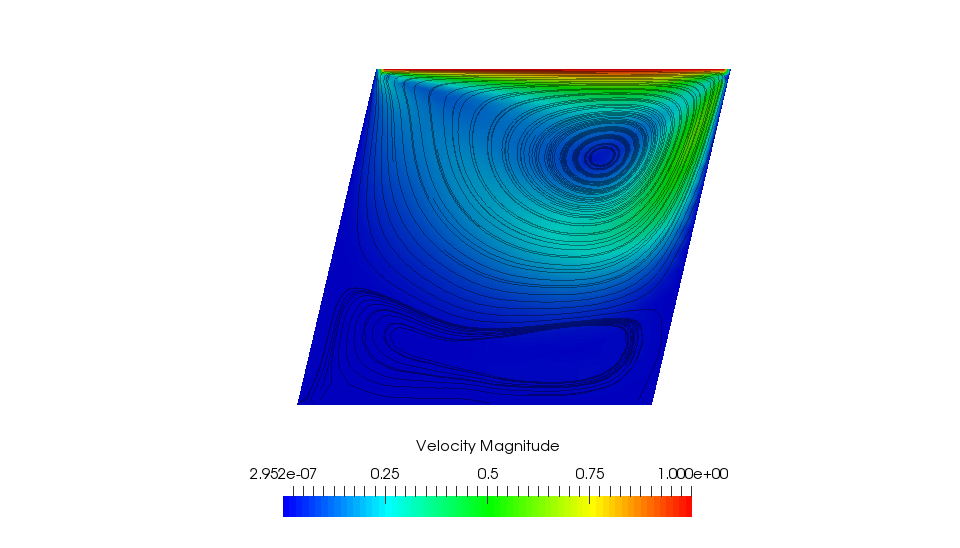
\includegraphics[scale = 0.4, trim = {7.5cm 0 7.5cm 0}, clip]{dc_400_test2_proj}} \\
		\subfloat[POD-G]{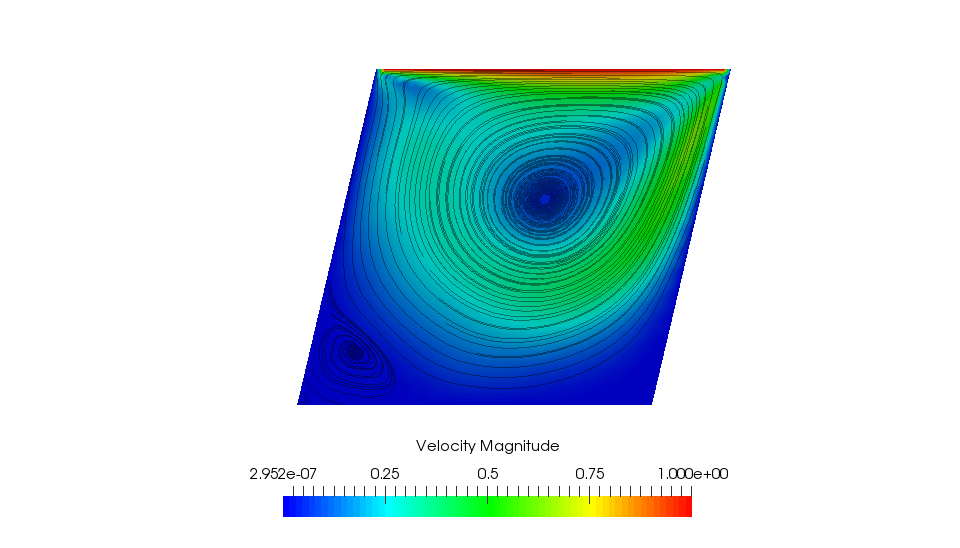
\includegraphics[scale = 0.4, trim = {7.5cm 0 7.5cm 0}, clip]{dc_400_test2_podg}}
		\subfloat[POD-N]{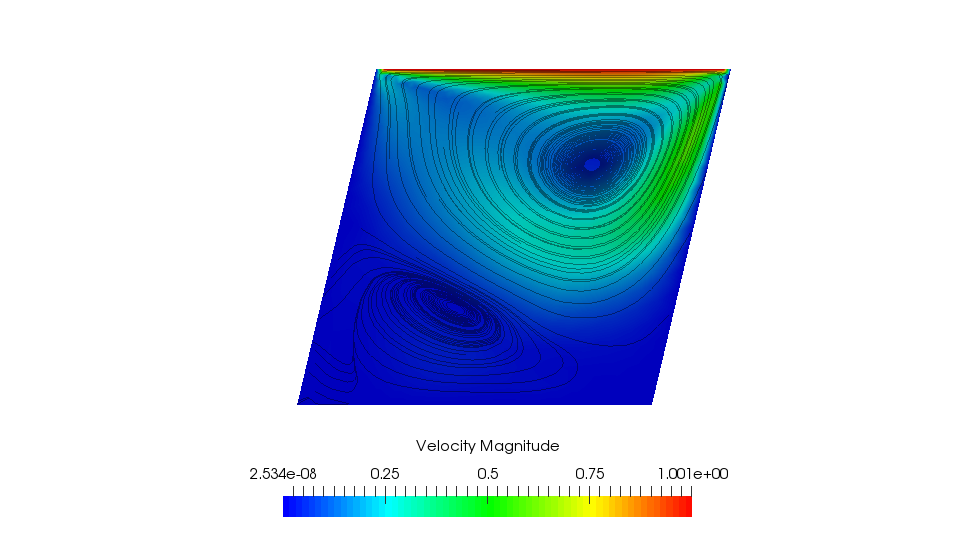
\includegraphics[scale = 0.4, trim = {7.5cm 0 7.5cm 0}, clip]{dc_400_test2_podnn}}
	\end{figure}
	
	\begin{figure}[H]
		\center
		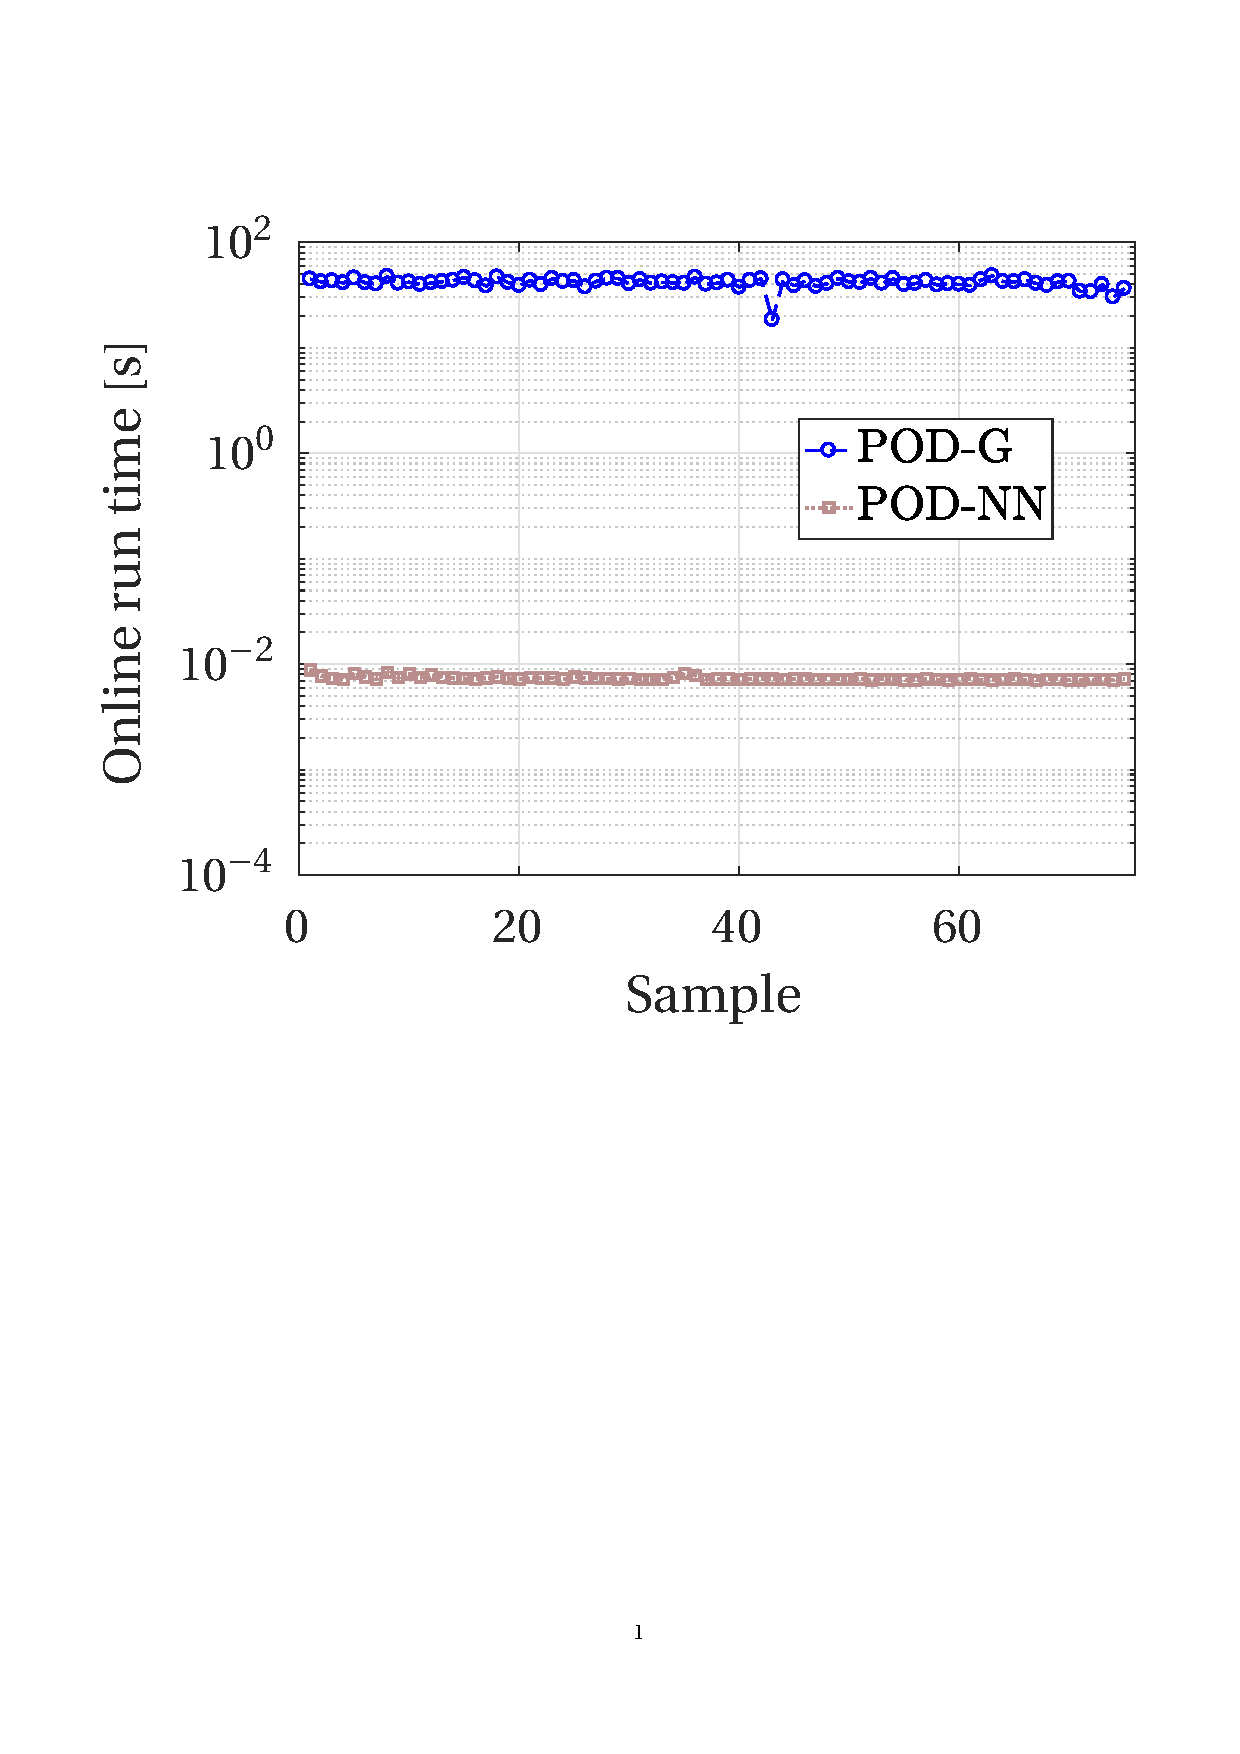
\includegraphics[scale = 0.75, trim = {1.5cm 11cm 1cm 3.5cm}, clip]{dc_400_time}
	\end{figure}
	
\end{document}
